\chapter{TileCal PMT response in calibration transfer analysis}
\label{app:pmt}

\section{Luminosity calibration transfer}

The general strategy to measure the luminosity in \gls{atlas} is outlined in Section \ref{sec:lumimeas}.
LUCID is the \gls{atlas} detector that, during \gls{vdm} runs, measures the absolute luminosity. 
LUCID algorithms are non-linear with $\mu$, and this non-linearity is corrected with the calibration transfer, 
that 
allows to extrapolate the absolute LUCID calibration from conditions corresponding to few low-$\mu$, isolated bunches 
to the conditions of the physics runs, where we have many high-$\mu$ bunches in trains. 

The default system used to provide the calibration transfer is track. As already discussed in Section \ref{sec:lumimeas},
the number of reconstructed tracks in the \gls{id} is proportional to $\mu$. 
The track selection that is used for the calibration transfer corresponds to the TightPrimary quality criteria but dropping 
the requirement on the Pixel holes (that have to be $\leq 1$ for the standard TightPrimary selection);
furthermore there is a requirement on the impact parameter significance, $|d_0|/\sigma(d_0)<7$, and on 
the pseudorapidity of the track, $|\eta|<1$. These criteria have been optimized to reduce the dependence on the Pixel conditions. 

The procedure to determine the calibration transfer assumes that the tracking luminosity measurement 
does not have any dependence on $\mu$ or on the position in the train, and it consists of three steps:
\begin{enumerate}
\item The bunch-averaged track luminosity during the \gls{vdm} run is normalized to the LUCID luminosity (which in these runs 
undergo the absolute calibration). The \gls{vdm} runs have low-$\mu$ isolated bunches.
\item The ratio of the luminosity measured by LUCID and track is measured as a function of $\mu$ (as measured by LUCID) 
in a single run with high-$\mu$ trains. The distribution of the values of this ratio is fitted with a straight line.
\item The result of the fit is used to apply a correction to the luminosity measured by LUCID in physics runs. 
%Fit the relative mu-dependence between the two in a single calibration-transfer run with high-mu trains. In the plot: x-axis mu measured by lucid. y: ratio of track to lucid luminosity. Fit the line. The mu dependence corresponds to an 11\% correction at mu=50 to the lucid response. This is a large number that we have to control at sub-percent level. 
%Apply to LUCID in physics runs 
\end{enumerate}

\begin{figure}[ht]
\centering
\subfigure{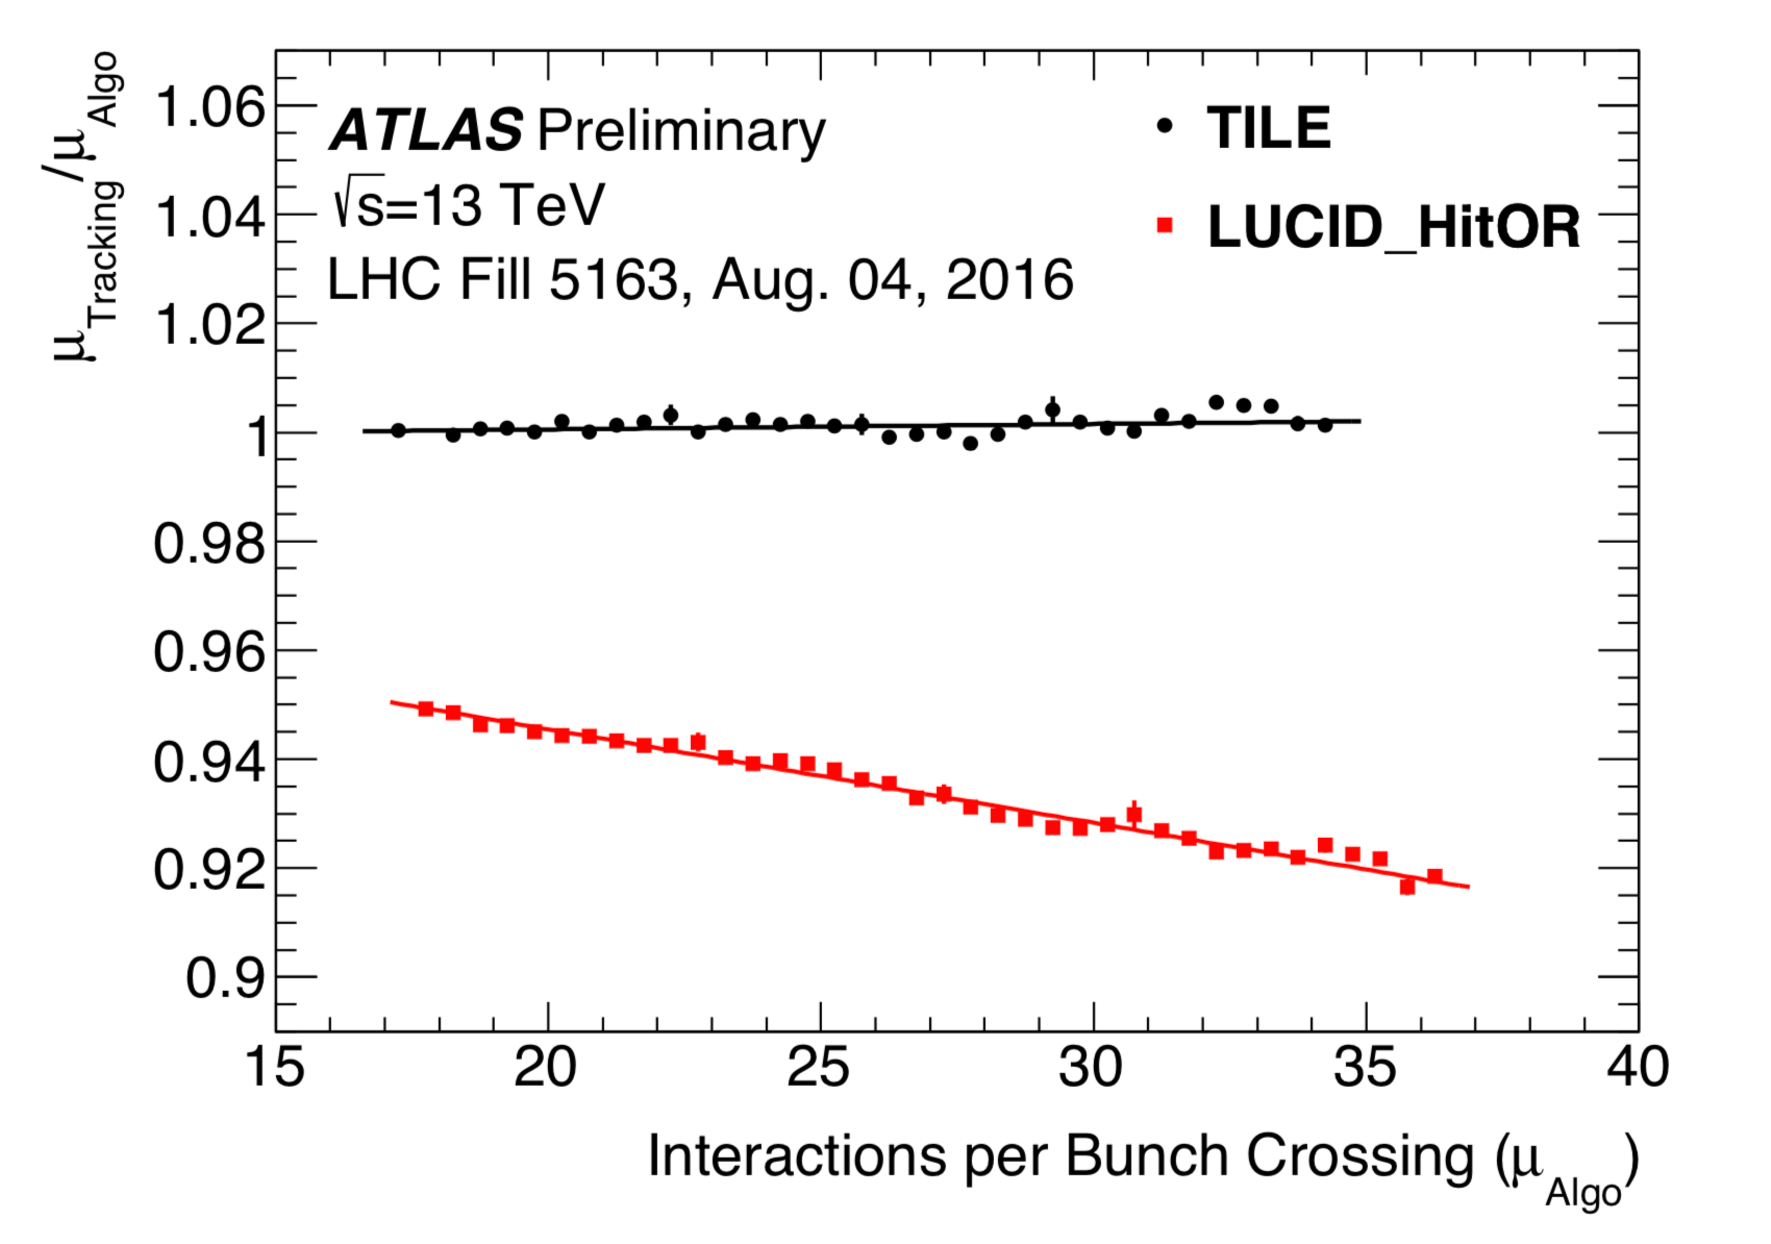
\includegraphics[width=0.65\textwidth]{figures/pmt_response/calibration_transfer_track.pdf}}
\caption{Ratio of the luminosity measured by LUCID (red) and \gls{tilecal} (black) to the track luminosity as a function of $\mu$.}
\label{fig:apppmt:calib_transfer}
\end{figure}

As it can be observed in Figure \ref{fig:apppmt:calib_transfer}, at high-$\mu$ LUCID overestimates the luminosity and 
the correction factor is as big as 11\% for $\mu \approx 50$. 

To assign an uncertainty to the calibration transfer, a similar procedure as what done with track is repeated using the 
integrator system of the \gls{tilecal} detector, and the relative difference between the luminosity measured by the tracking system and 
by \gls{tilecal}  is used as uncertainty. 
Just like in the case of the luminosity measurement from the tracking system, the \gls{tilecal} luminosity measurement 
relies on some assumptions, in particular perfect linearity of the \gls{pmt} response over a wide range of instantaneous luminosity, 
that spans over three order of magnitude. 
The cells considered are all the E-type cells and A13.
The difference between the track and the \gls{tilecal} measurement of the calibration transfer is performed as follows:
\begin{enumerate}
\item The luminosity of all the \gls{tilecal} cells used is individually calibrated to match the track luminosity 
at a specific high-$\mu$ run (anchor run).
\item Interpolating this value with the origin in the current-luminosity plane allows to derive an estimate for the \gls{tilecal} 
luminosity during the \gls{vdm} run.
\item The comparison of this luminosity with the luminosity measured by the tracking system provides the systematic uncertainty on the 
calibration transfer. 
\end{enumerate}
The measurement of the calibration transfer with \gls{tilecal} needs to take into account two effects that complicate the measurement. 
\begin{itemize}
\item Activation decays after high-$\mu$ runs bias the \gls{tilecal} response in low-$\mu$ runs like the \gls{vdm} run.
\item It has been shown that the \gls{pmt} response is not perfectly linear with the luminosity. 
\end{itemize}

The next two sections focus on the analysis of this second point and on the corrections derived to minimize its effect 
on the \gls{tilecal} calibration transfer analysis; this allows to reduce the calibration transfer uncertainty on the 
2017 luminosity, which is the dominant luminosity uncertainty for the 2016 dataset. 


\section{PMT response in empty bunches}
\label{sec:app:pmtresponse}

It has previously been noticed (e.g. Ref. \cite{giulia:tesi}) that the \gls{tilecal} \gls{pmt} show a non-linearity in 
the response with the increase in luminosity. 
In this section we study this effect for the cells and the run numbers that are of interest for the 
calibration transfer analysis. 

The \gls{tilecal} laser system is primarily used to calibrate the \gls{tilecal} readout. 
The laser system can also be fired in the abort gaps during standard physics runs; in this case 
one laser pulse is sent three times per second.

The anchor run used in the calibration transfer analysis is 331085. 

The \gls{pmt} response is analyzed in the following steps:
\begin{enumerate}
\item The response of the \glspl{pmt} is normalized to the response of the monitor diode D0 to remove fluctuations 
due to laser instabilities.

\item The distribution of the response each individual \gls{pmt} in groups of 25 \gls{lb} is considered. 
Grouping together several \glspl{lb} is necessary to accumulate enough statistic: the frequency of laser pulses is 3 Hz, 
which gives us only about 180 data points per minute. The value of 25 has been chosen for consistency with previous studies, 
after checking that the size of the group of \glspl{lb} does not to affect the results 
as long as it is large enough to provide sufficient statistic.

\item The response for each cell family is computed by averaging over all the \glspl{pmt} 
belonging to that family. We keep separate the left and right \glspl{pmt} and the A and C side 
of \gls{tilecal}

\item The distribution of the response is normalized to the last group of \glspl{lb} that 
does not contain the \gls{lb} where "stable beams" is declared, which is used as reference.

\end{enumerate} 

Figure \ref{fig:apppmt:331085:variation_A13} shows the \gls{pmt} response for the cell family A13 during the anchor run, 
while Figure \ref{fig:apppmt:331085:variation_E1_E2} shows the response for the cells of the families E1 and E2 
and Figure \ref{fig:apppmt:331085:variation_E3_E4} for the families E3 and E4.

\begin{figure}[htbp]
\centering
\subfigure{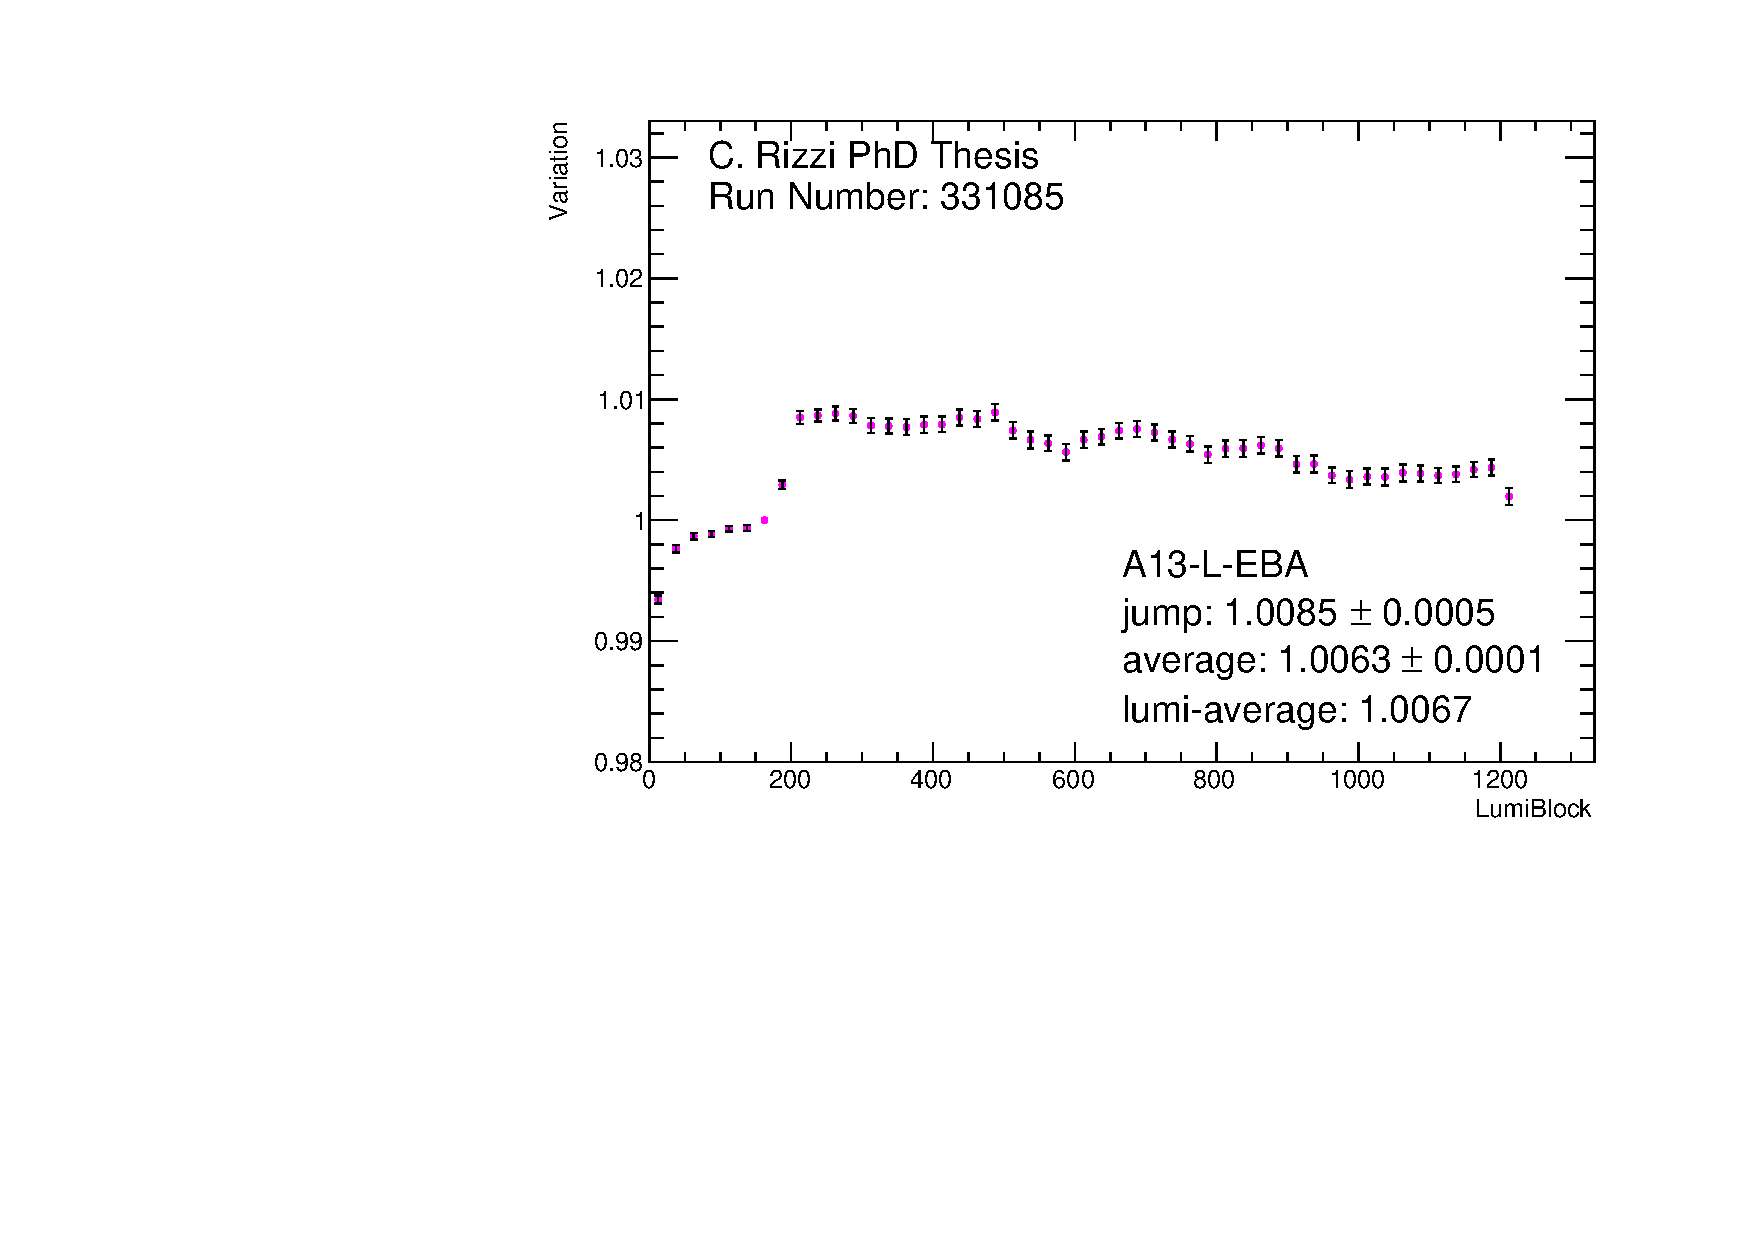
\includegraphics[width=0.45\textwidth]{figures/pmt_response/331085/variation_A13_L_EBA}\label{fig:app:variation_A13_L_EBA}}
\subfigure{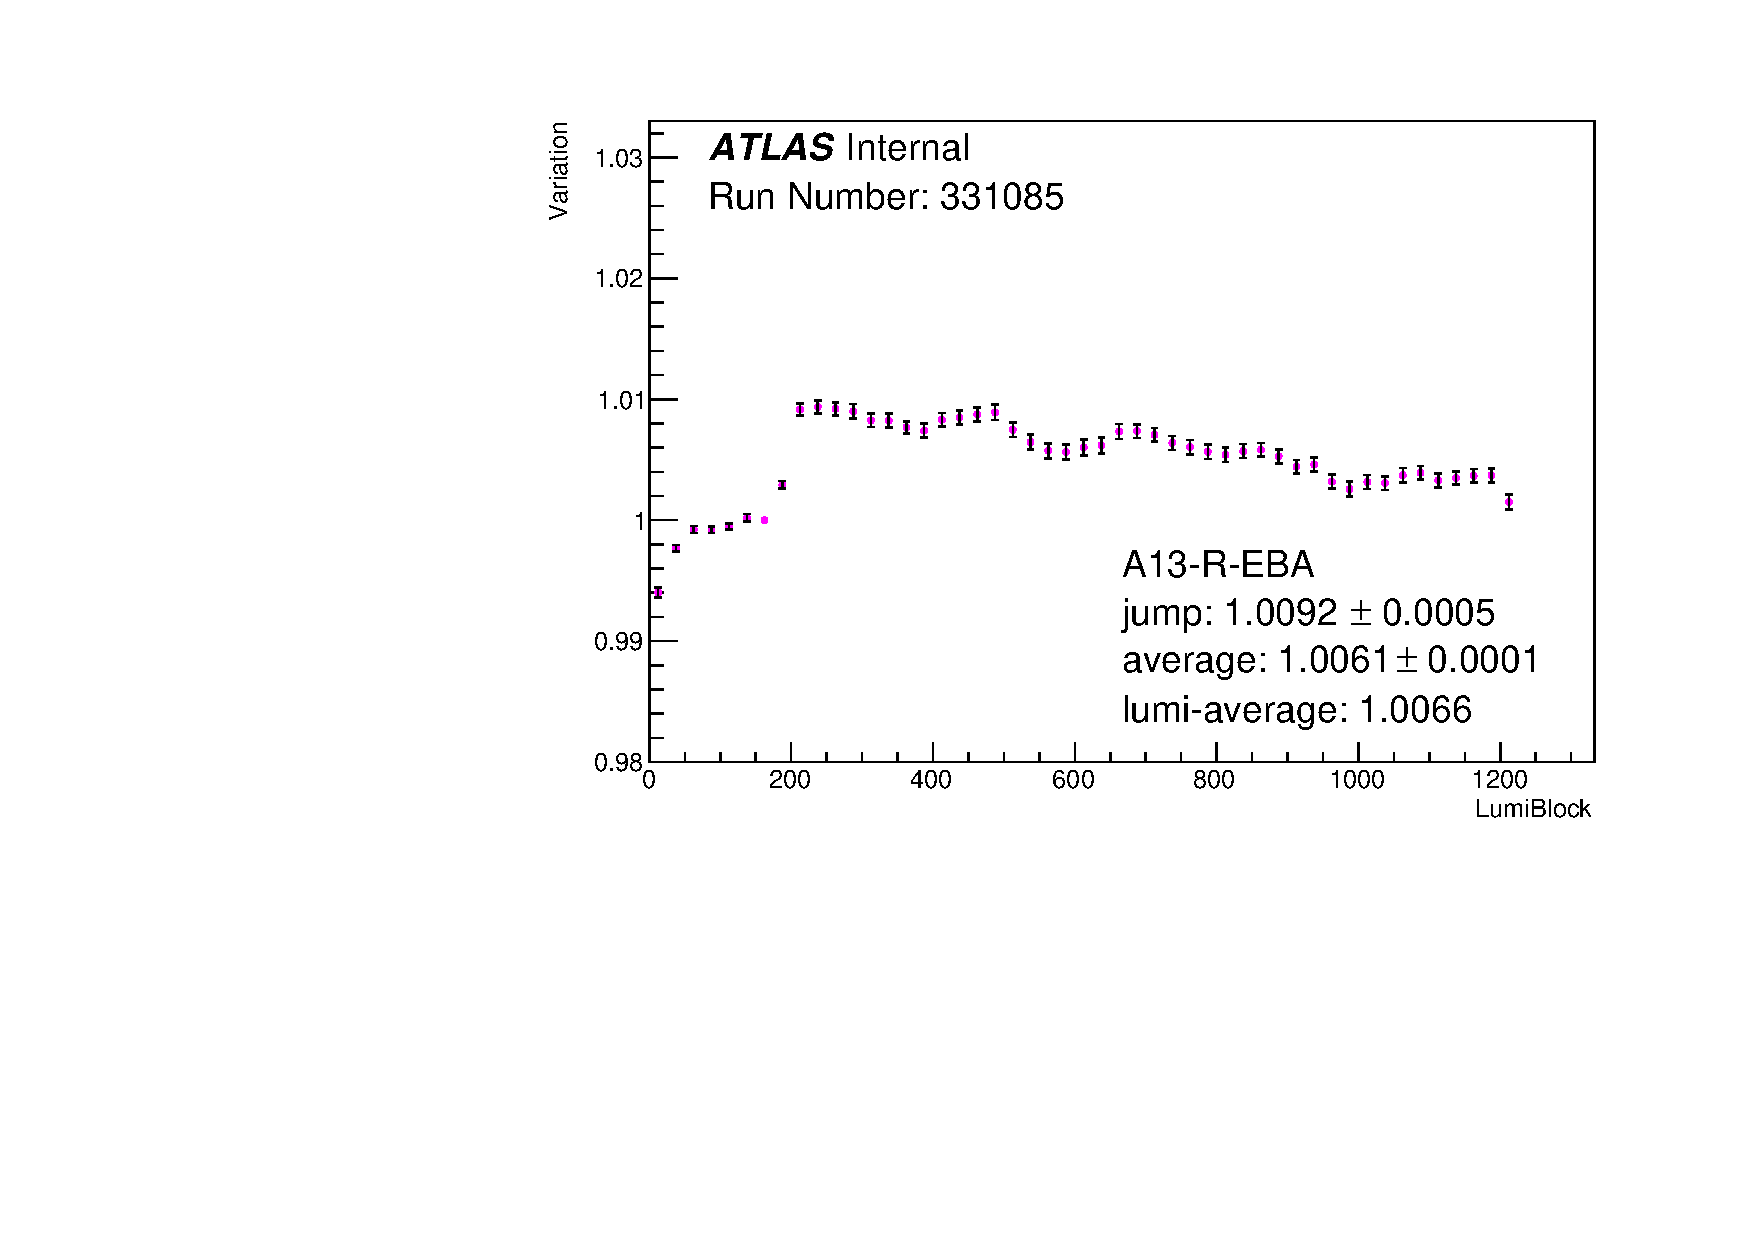
\includegraphics[width=0.45\textwidth]{figures/pmt_response/331085/variation_A13_R_EBA}\label{fig:app:variation_A13_R_EBA}}\\
\subfigure{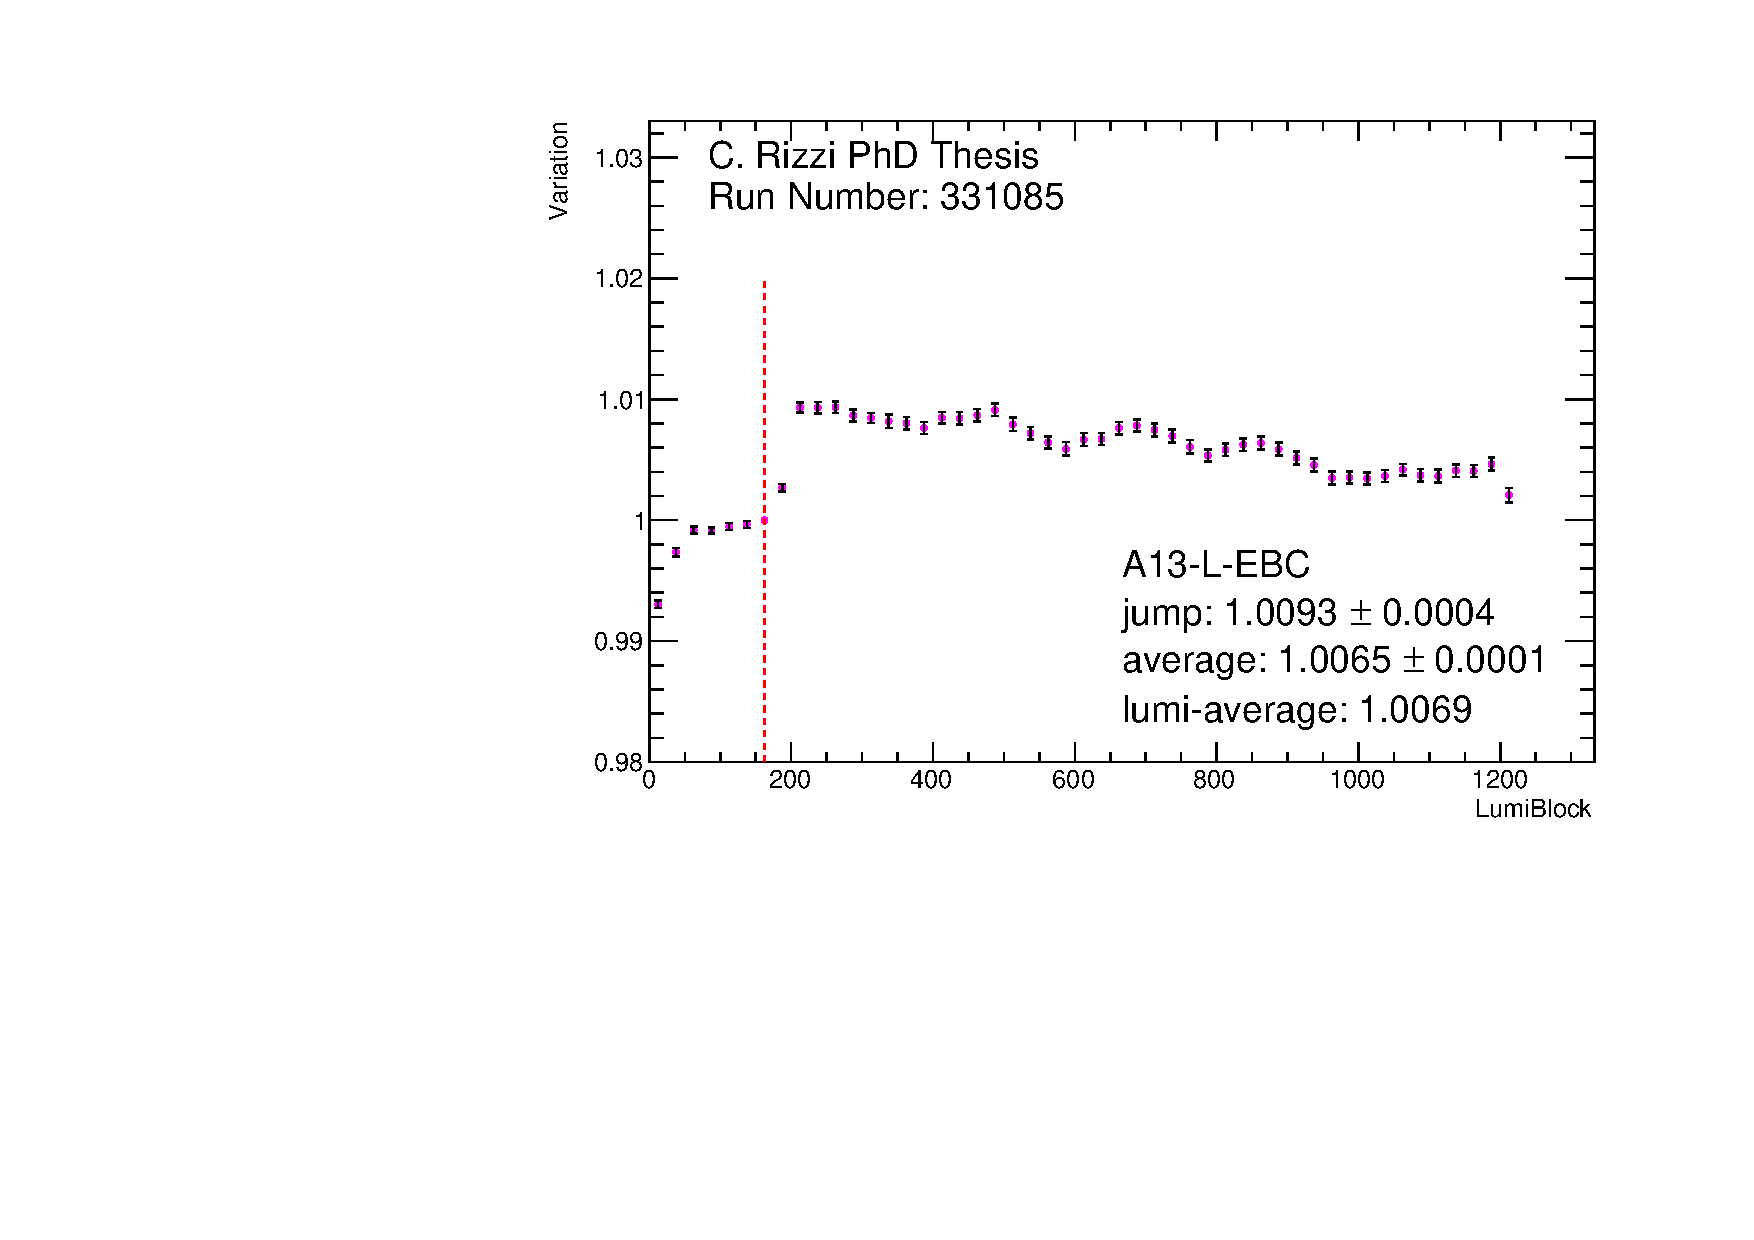
\includegraphics[width=0.45\textwidth]{figures/pmt_response/331085/variation_A13_L_EBC}\label{fig:app:variation_A13_L_EBC}}
\subfigure{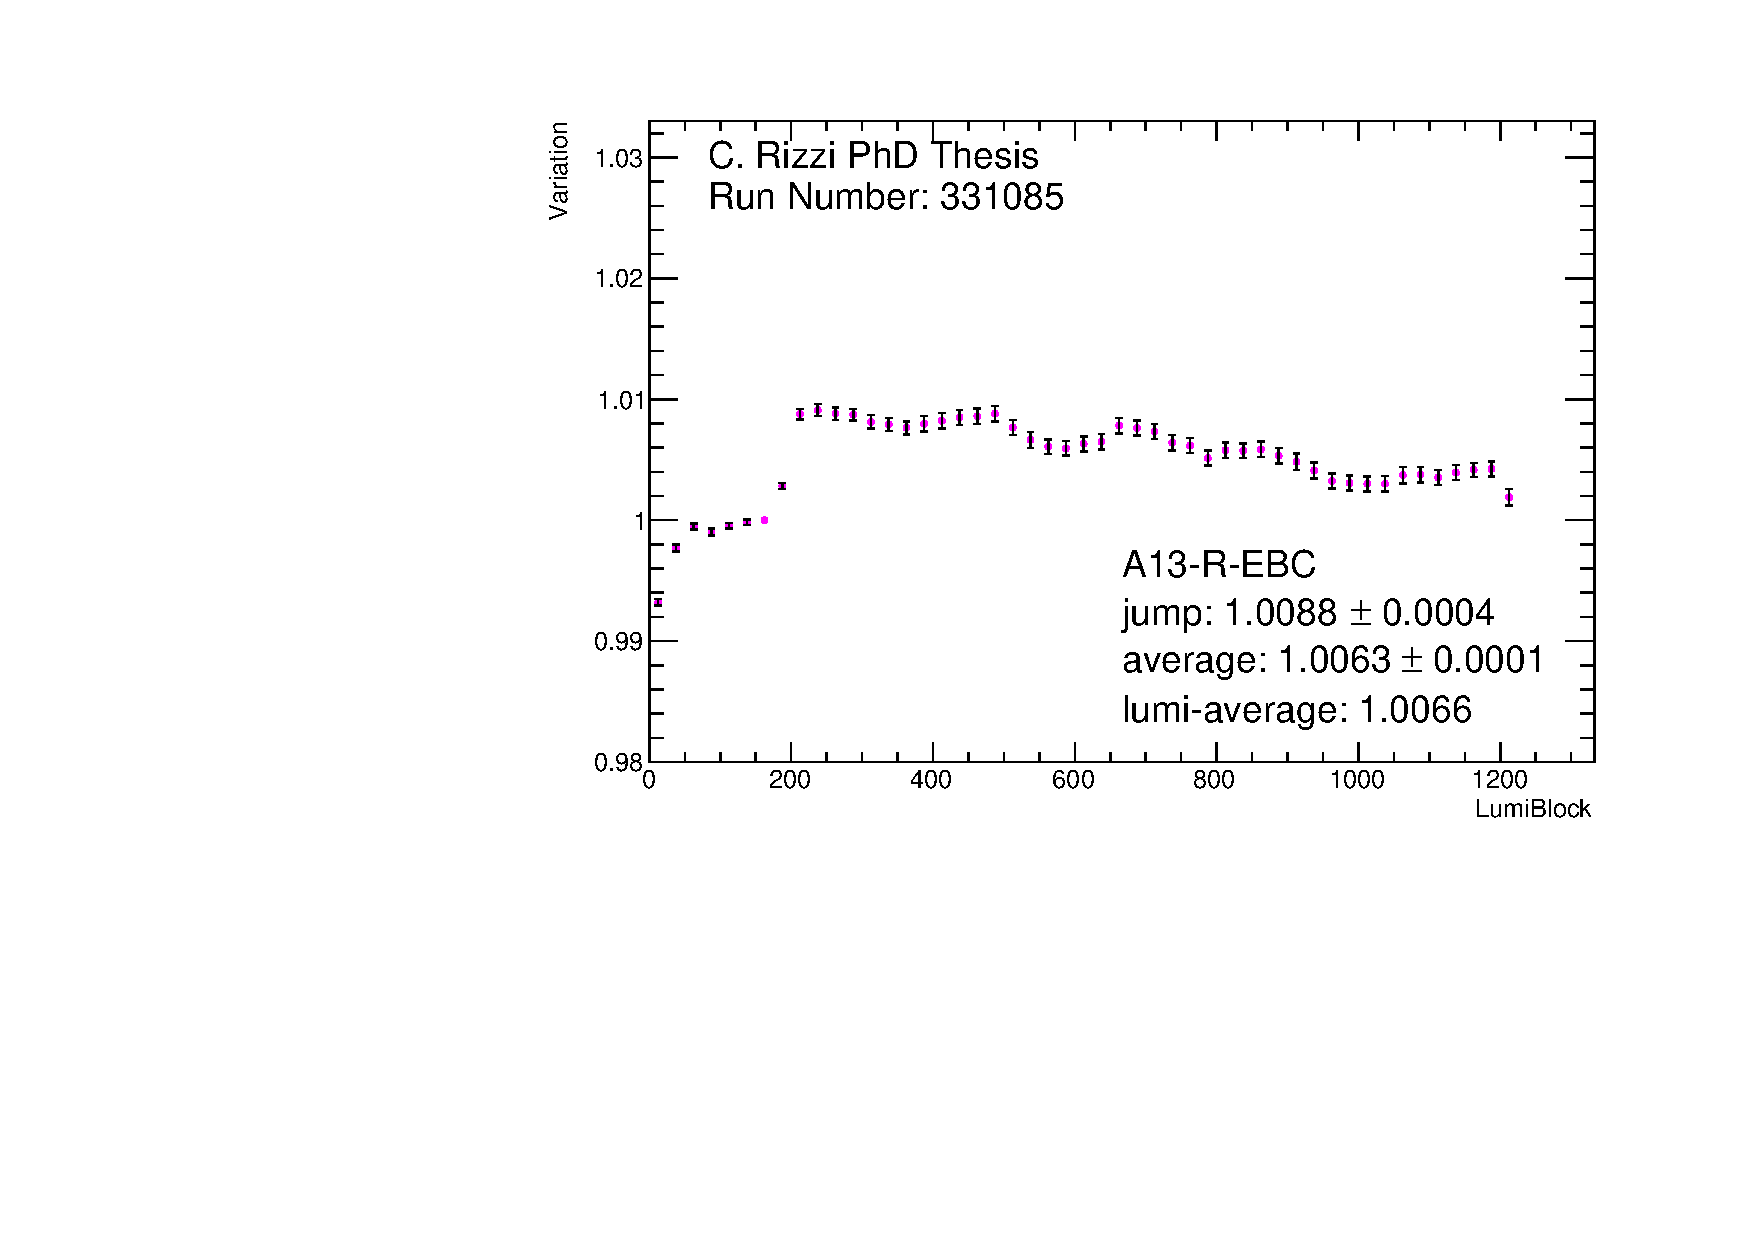
\includegraphics[width=0.45\textwidth]{figures/pmt_response/331085/variation_A13_R_EBC}\label{fig:app:variation_A13_R_EBC}}\\
\caption{\gls{pmt} response in cell A13 for the anchor run (run number 331085).}
\label{fig:apppmt:331085:variation_A13}
\end{figure}

\begin{figure}[htbp]
\centering
\subfigure{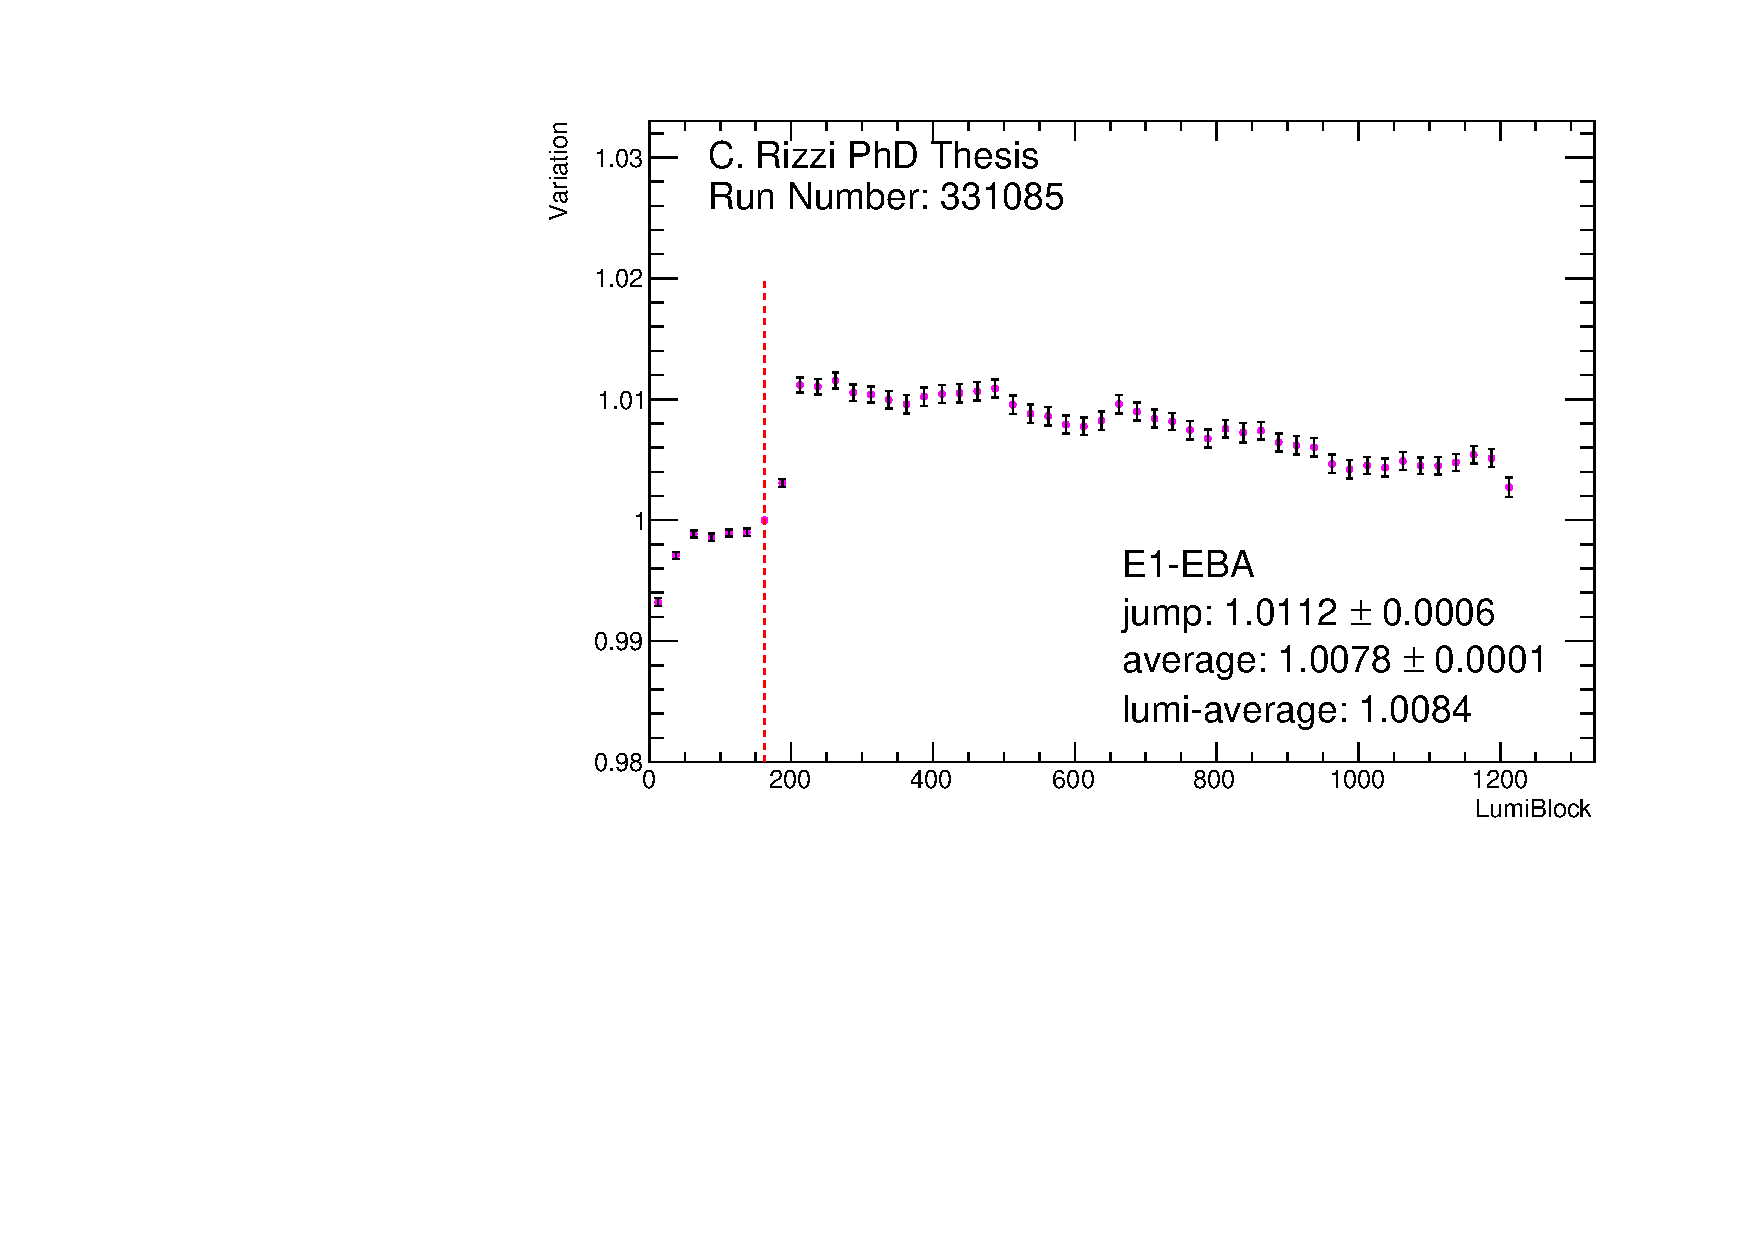
\includegraphics[width=0.45\textwidth]{figures/pmt_response/331085/variation_E1_EBA}\label{fig:app:variation_E1_EBA}}
\subfigure{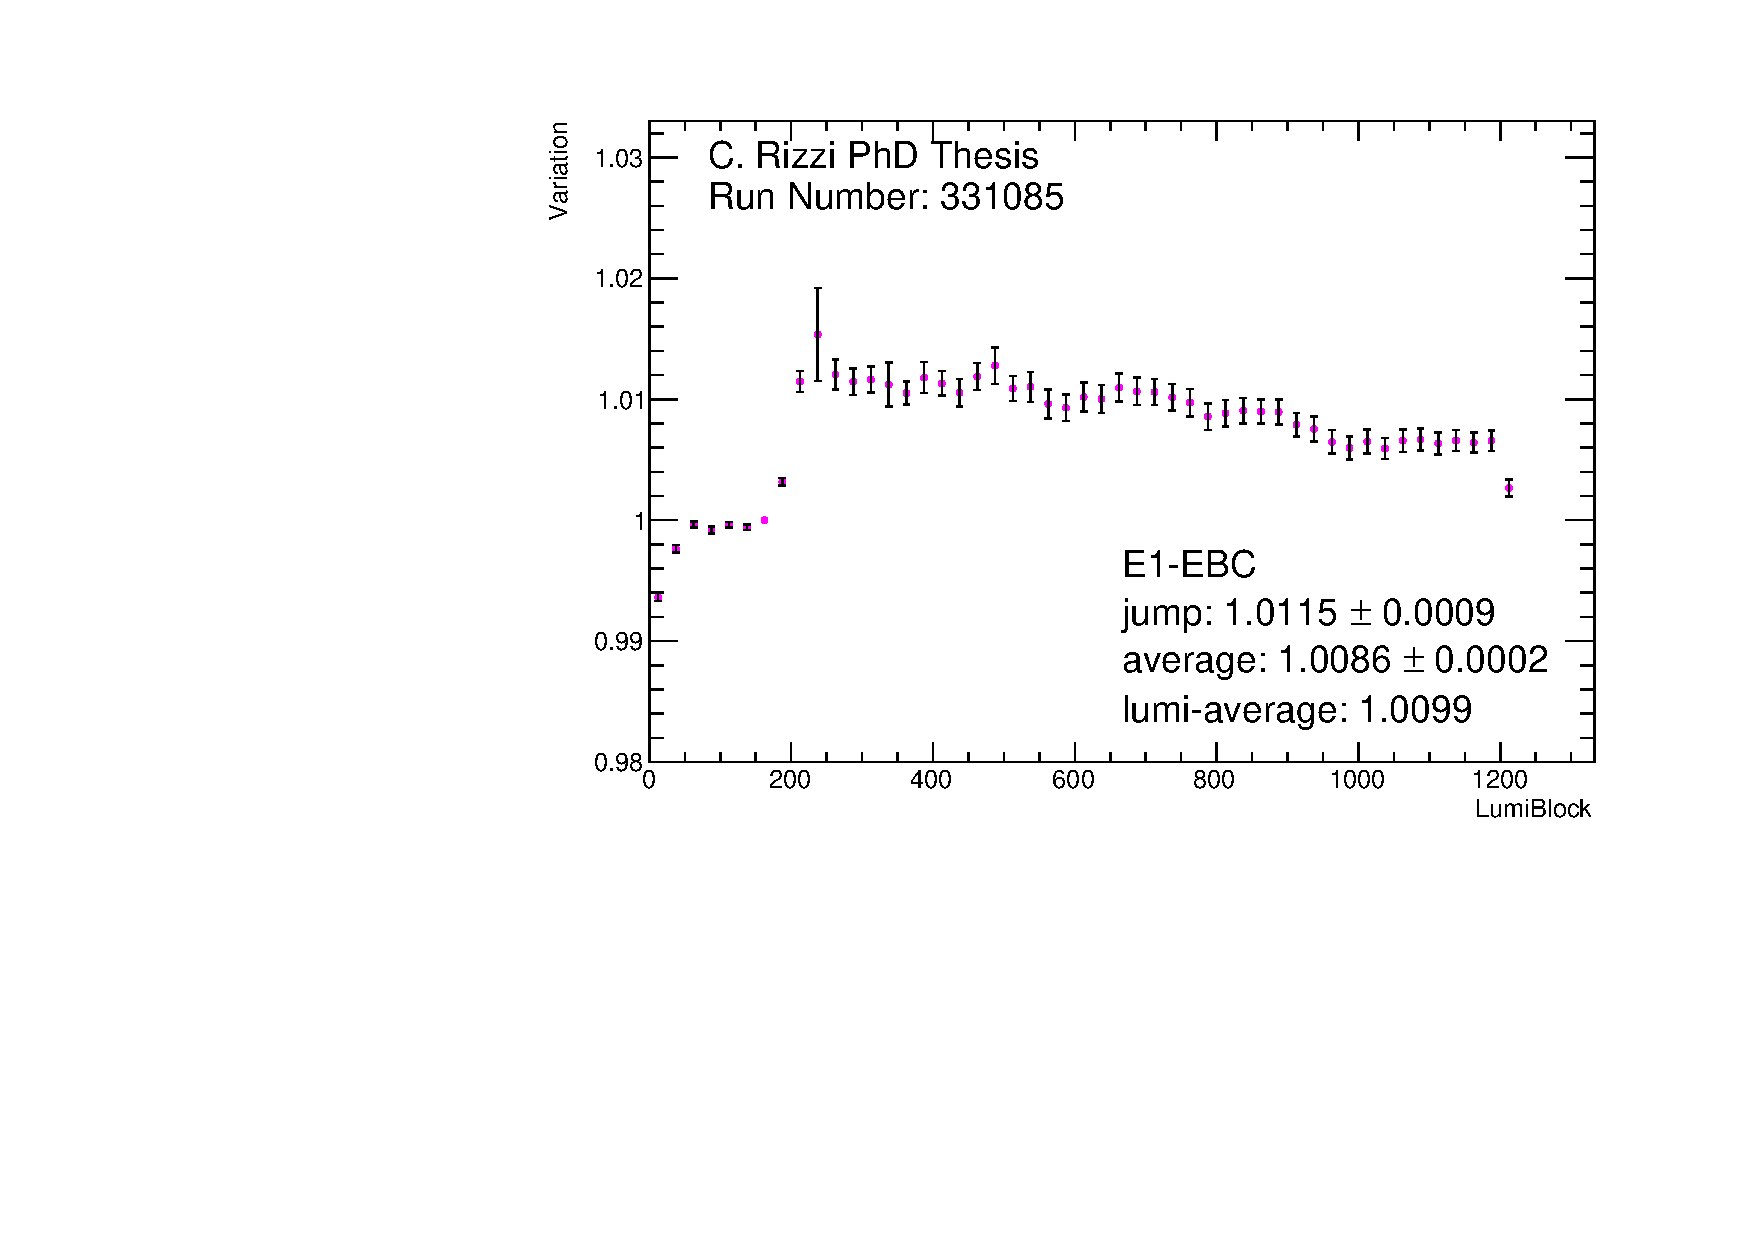
\includegraphics[width=0.45\textwidth]{figures/pmt_response/331085/variation_E1_EBC}\label{fig:app:variation_E1_EBC}}\\
\subfigure{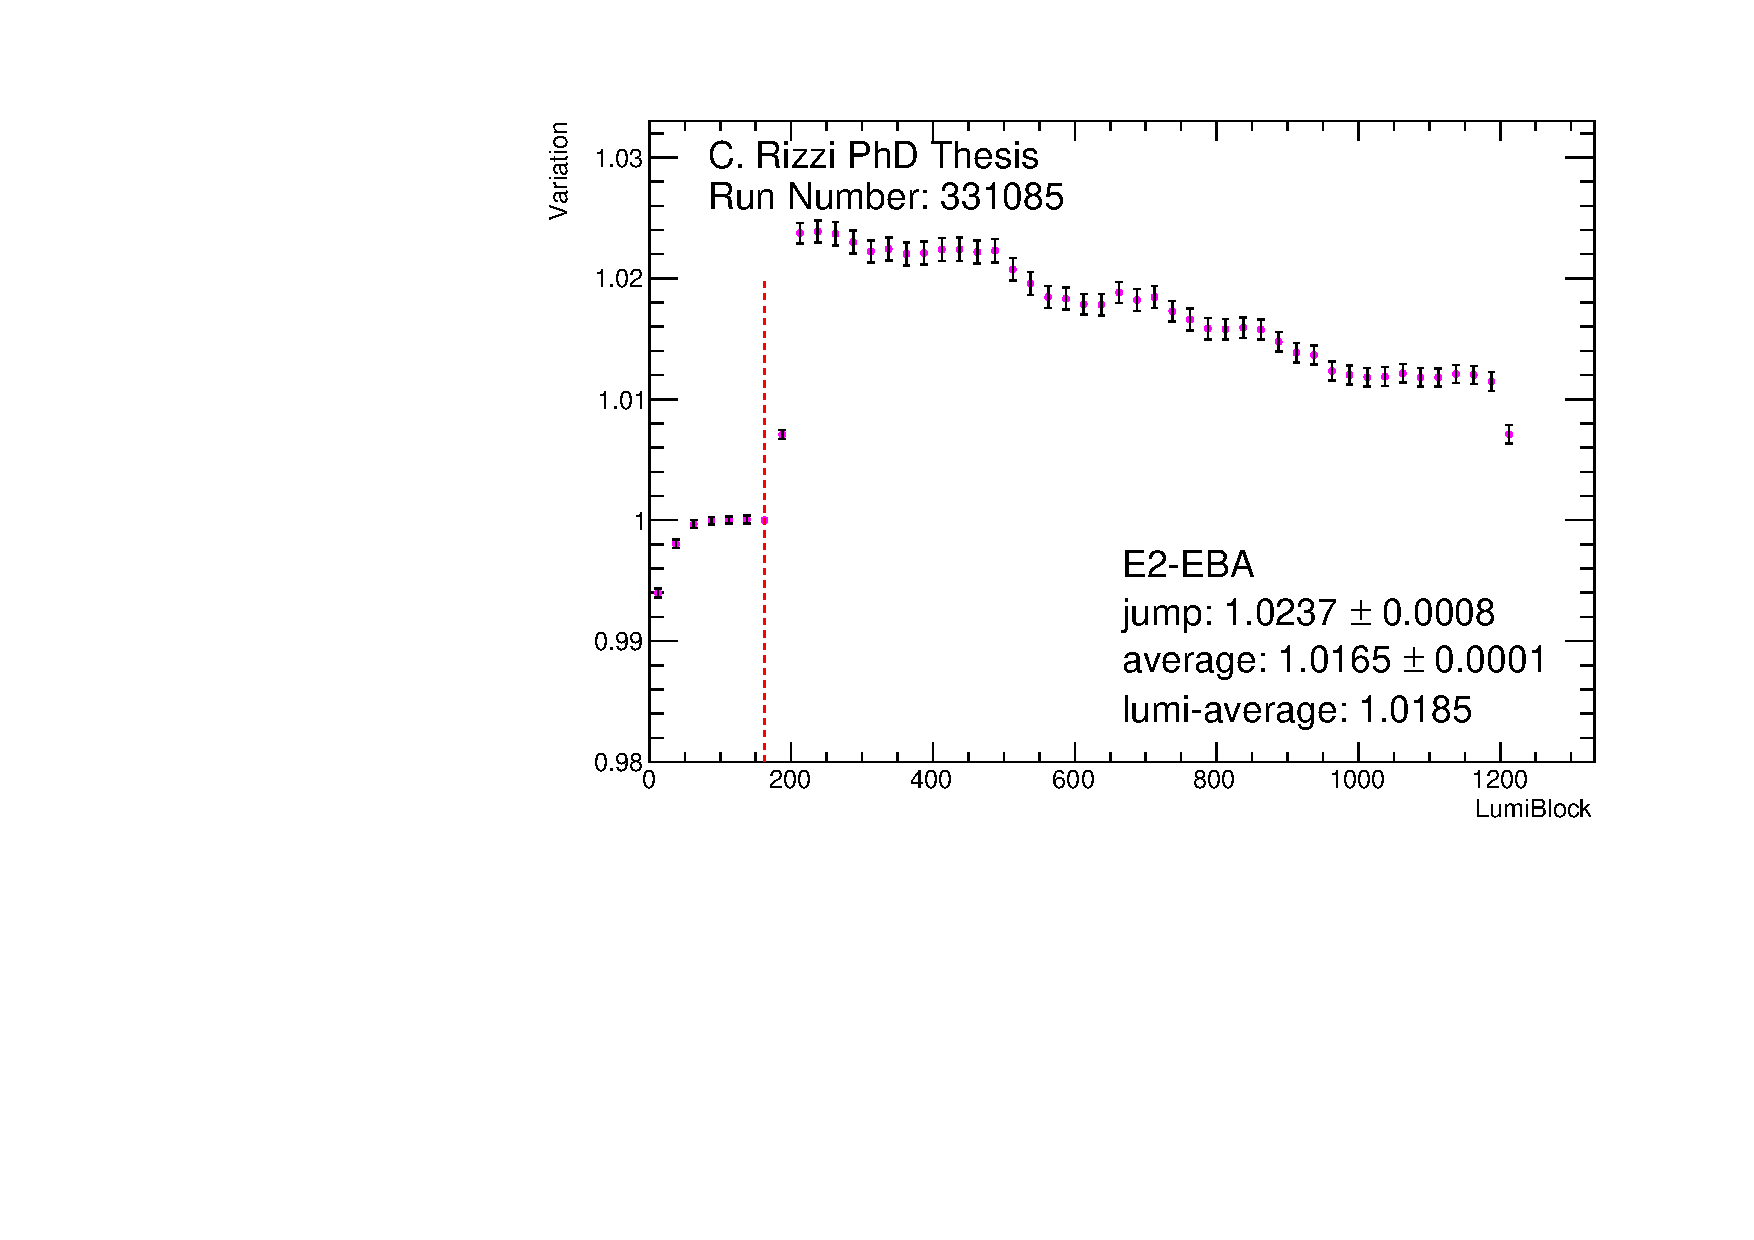
\includegraphics[width=0.45\textwidth]{figures/pmt_response/331085/variation_E2_EBA}\label{fig:app:variation_E2_EBA}}
\subfigure{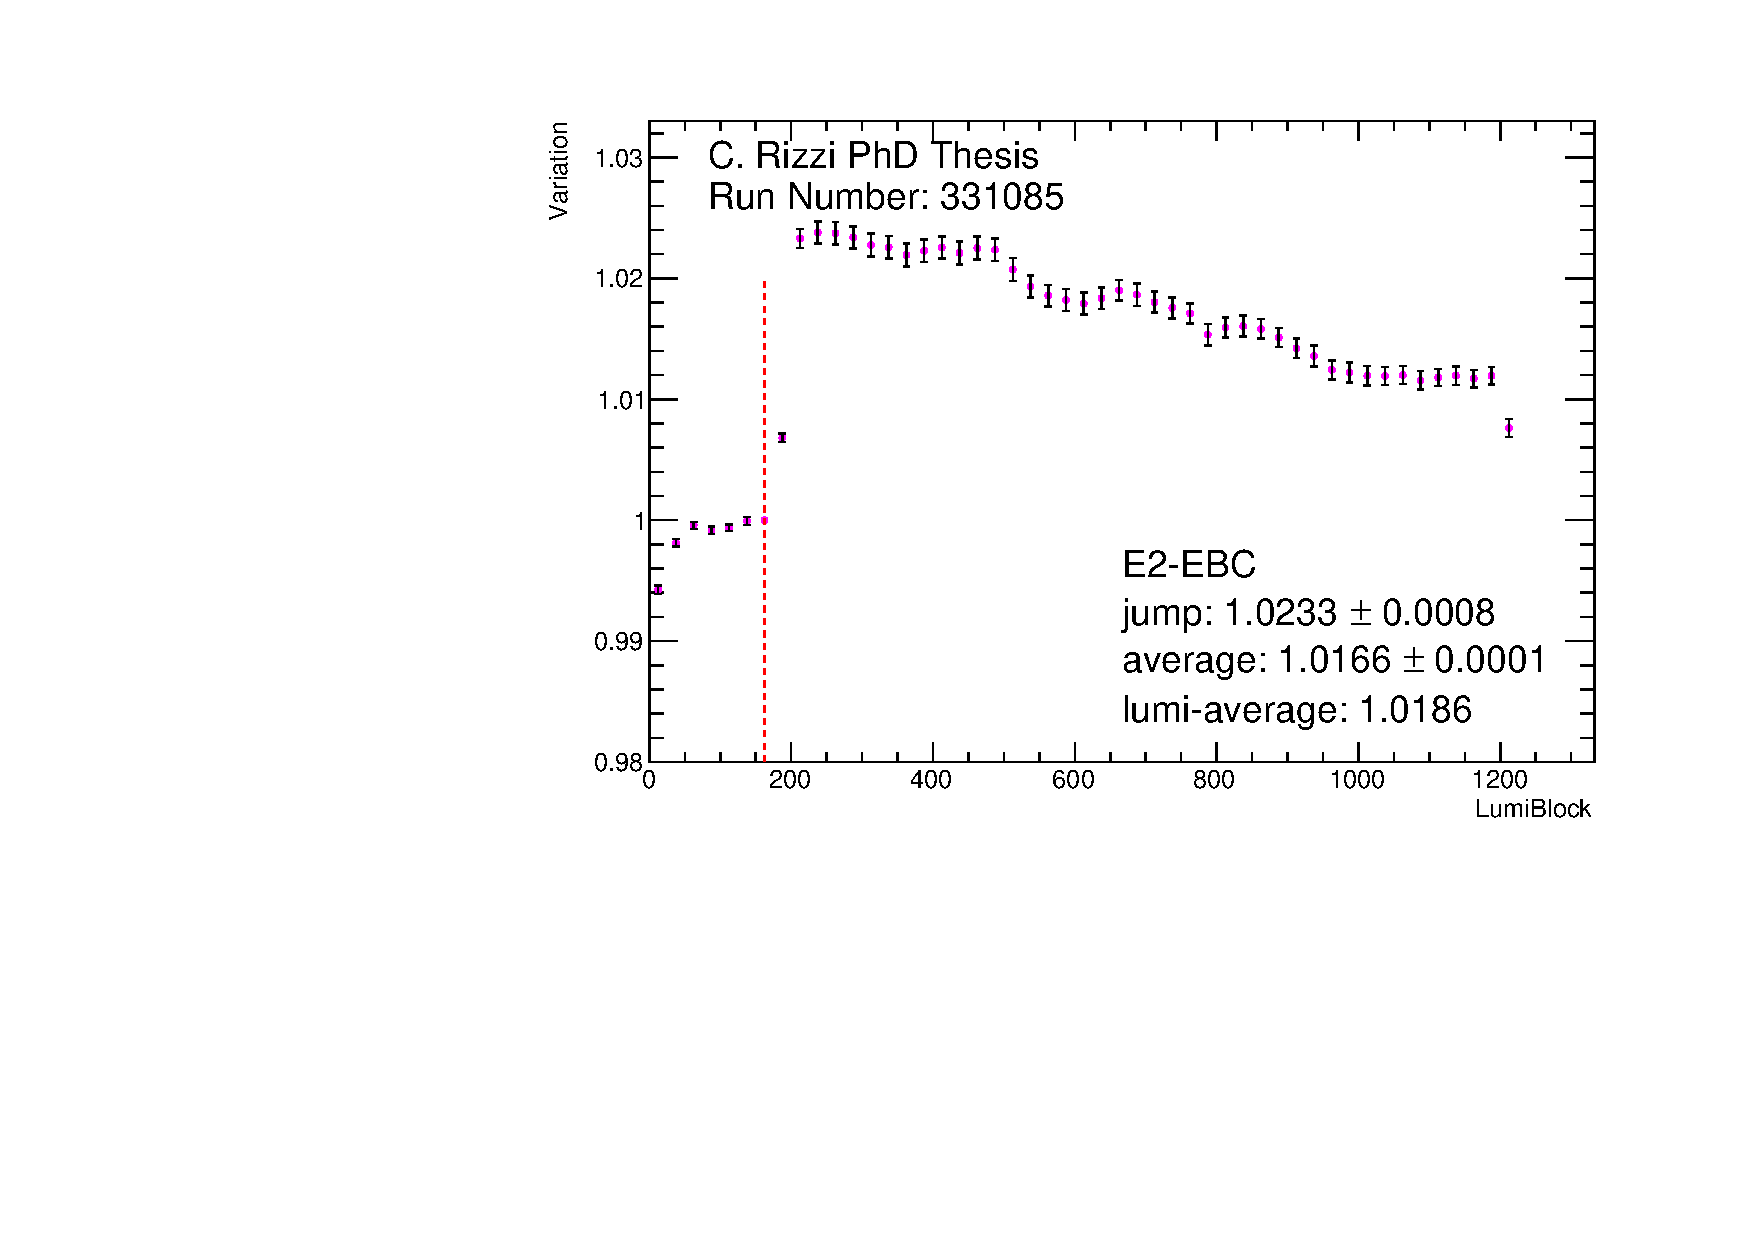
\includegraphics[width=0.45\textwidth]{figures/pmt_response/331085/variation_E2_EBC}\label{fig:app:variation_E2_EBC}}\\
\caption{\gls{pmt} response in cell E1 and E2 for the anchor run (run number 331085).}
\label{fig:apppmt:331085:variation_E1_E2}
\end{figure}

\begin{figure}[htbp]
\centering
\subfigure{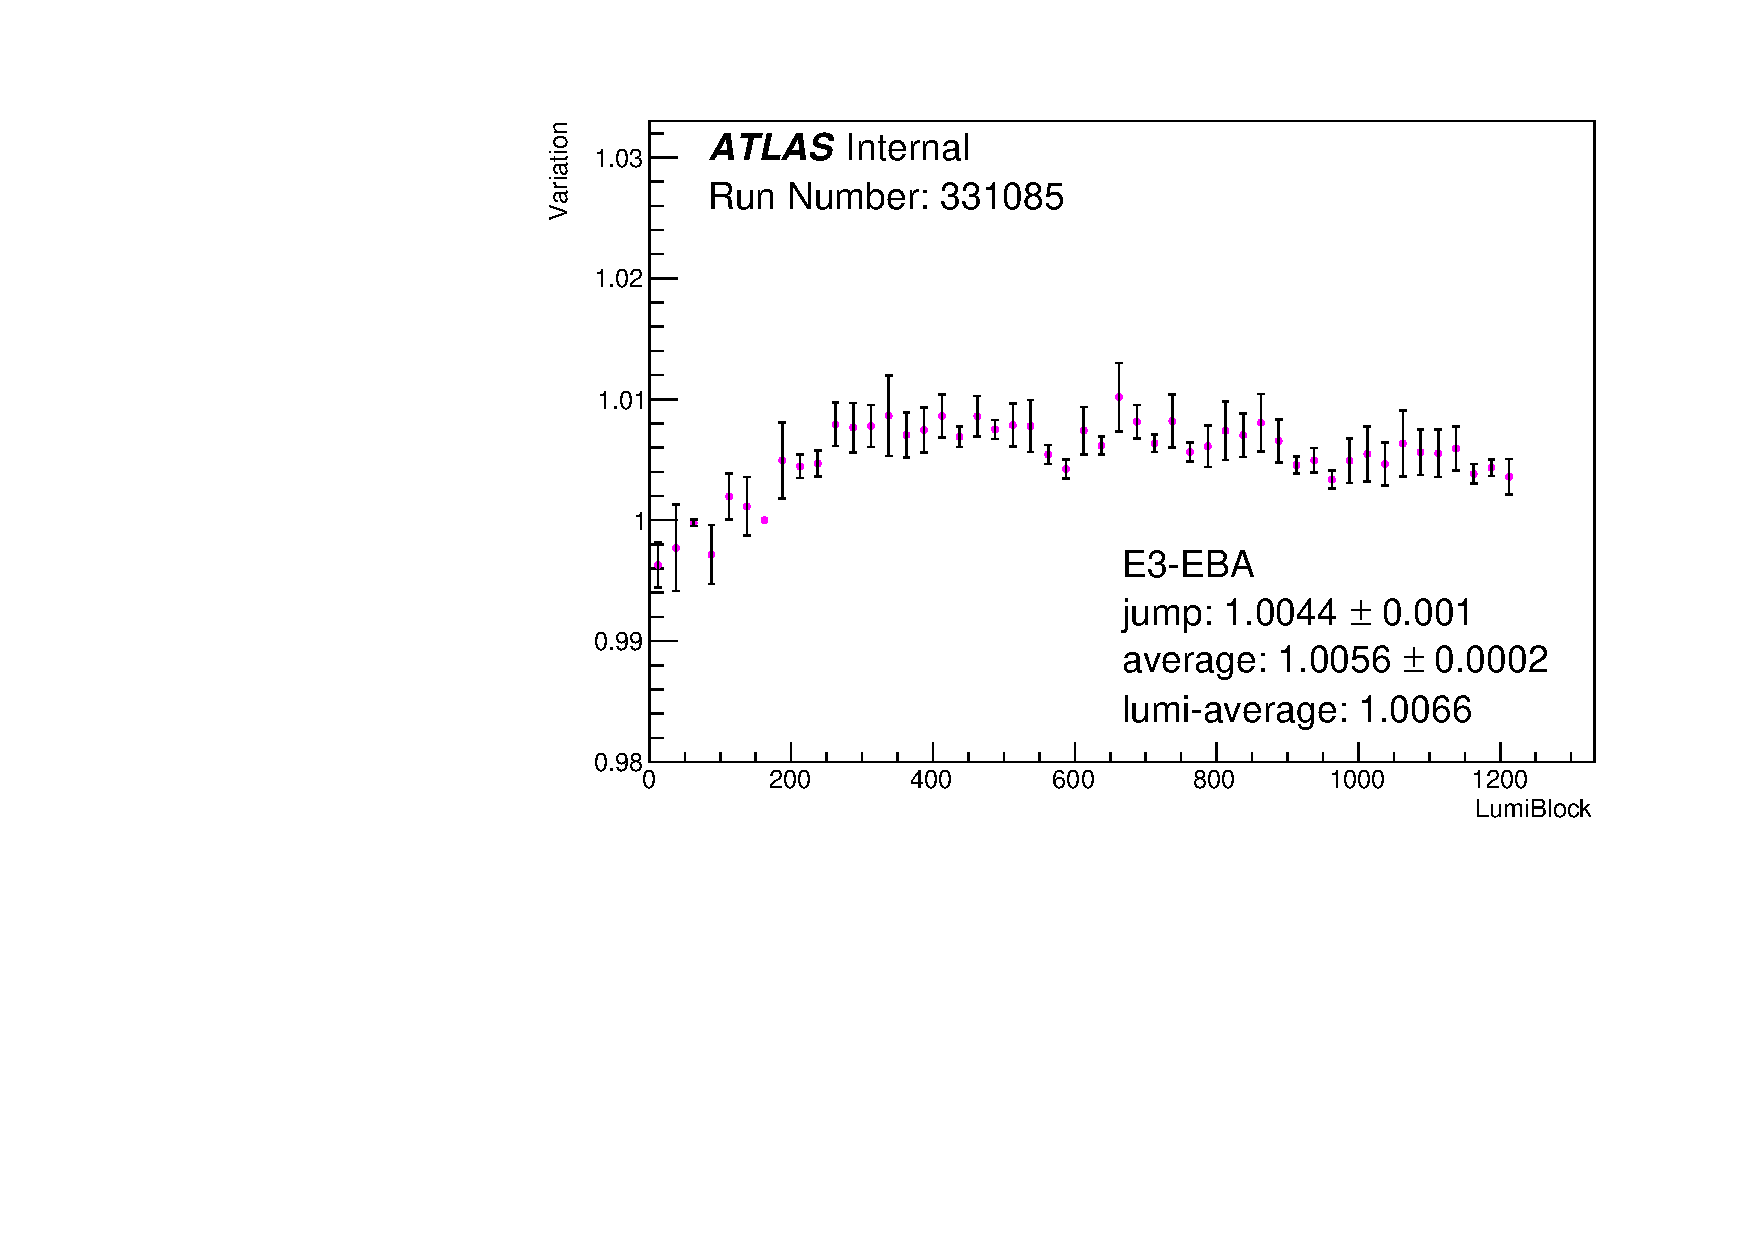
\includegraphics[width=0.45\textwidth]{figures/pmt_response/331085/variation_E3_EBA}\label{fig:app:variation_E3_EBA}}
\subfigure{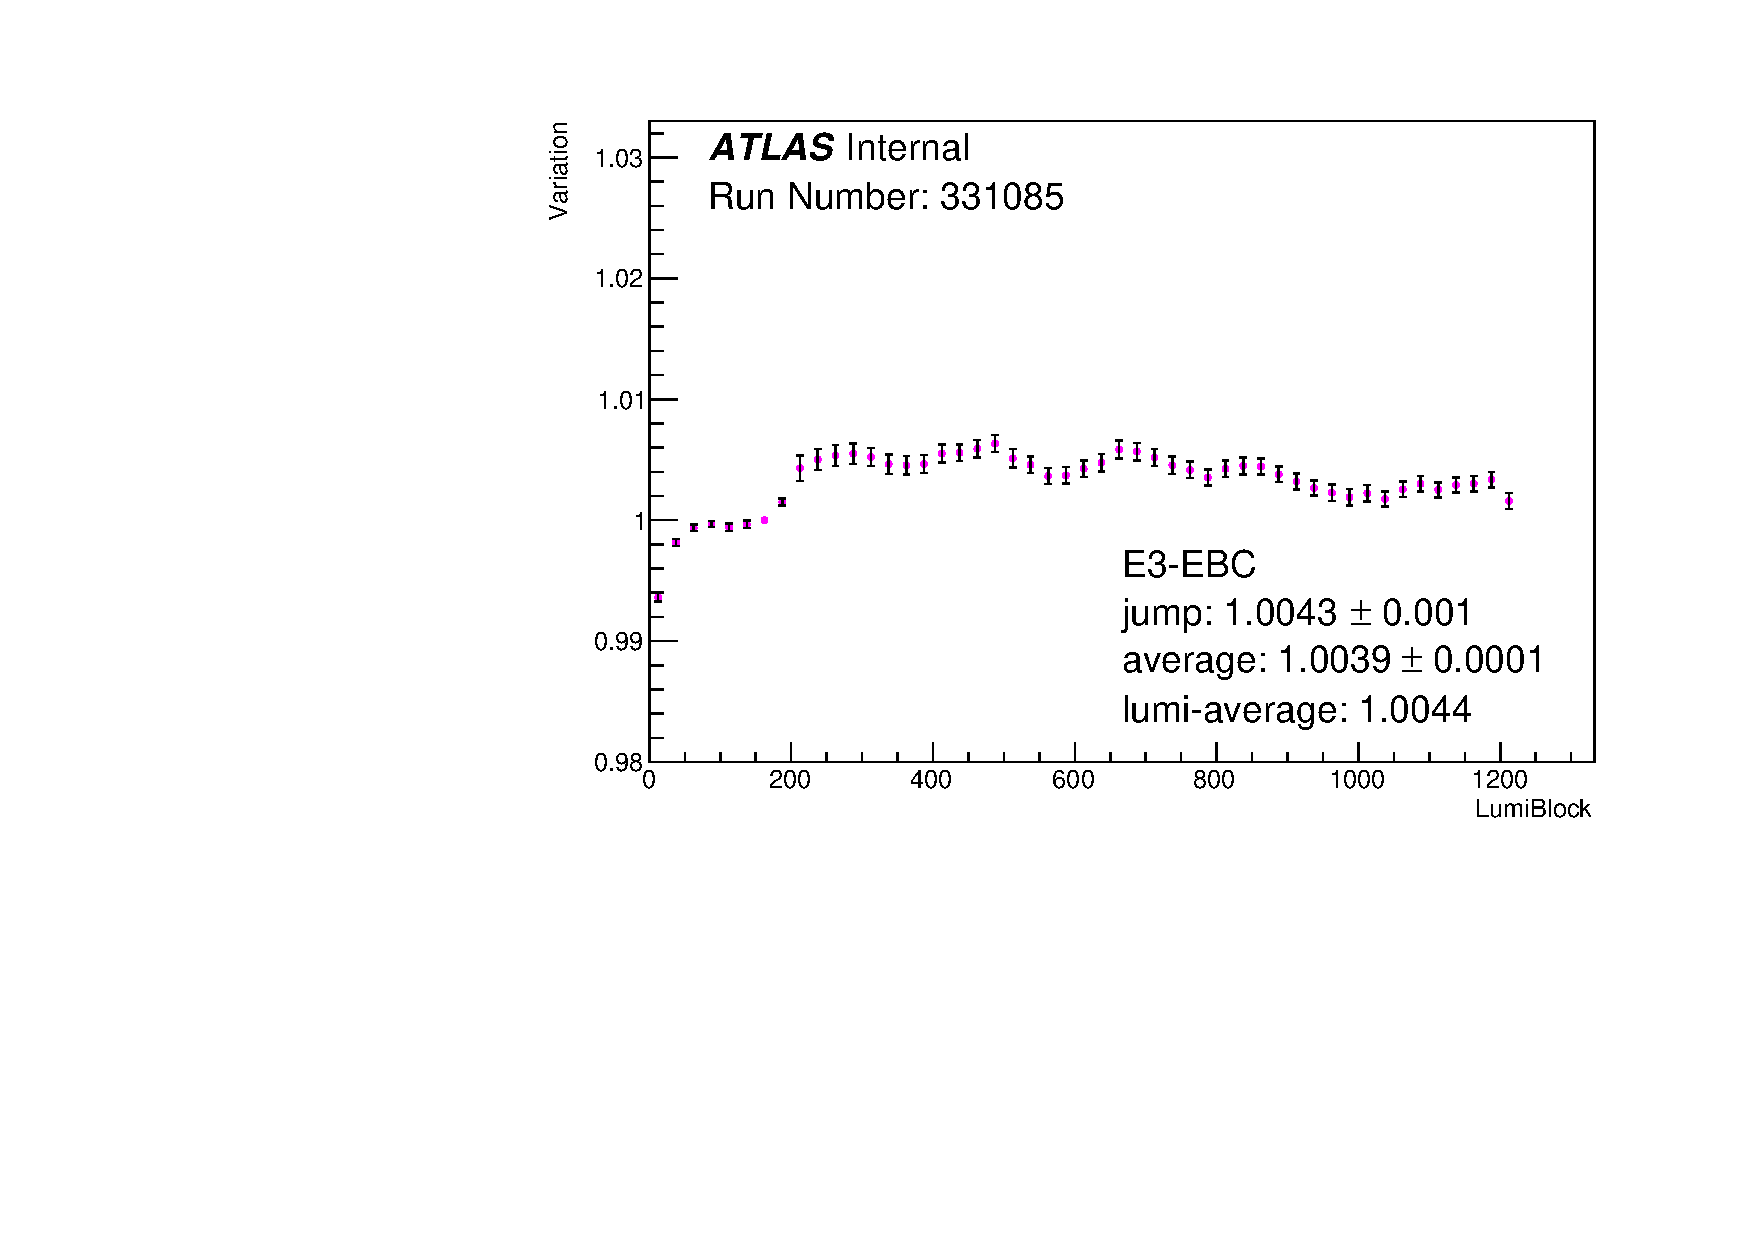
\includegraphics[width=0.45\textwidth]{figures/pmt_response/331085/variation_E3_EBC}\label{fig:app:variation_E3_EBC}}\\
\subfigure{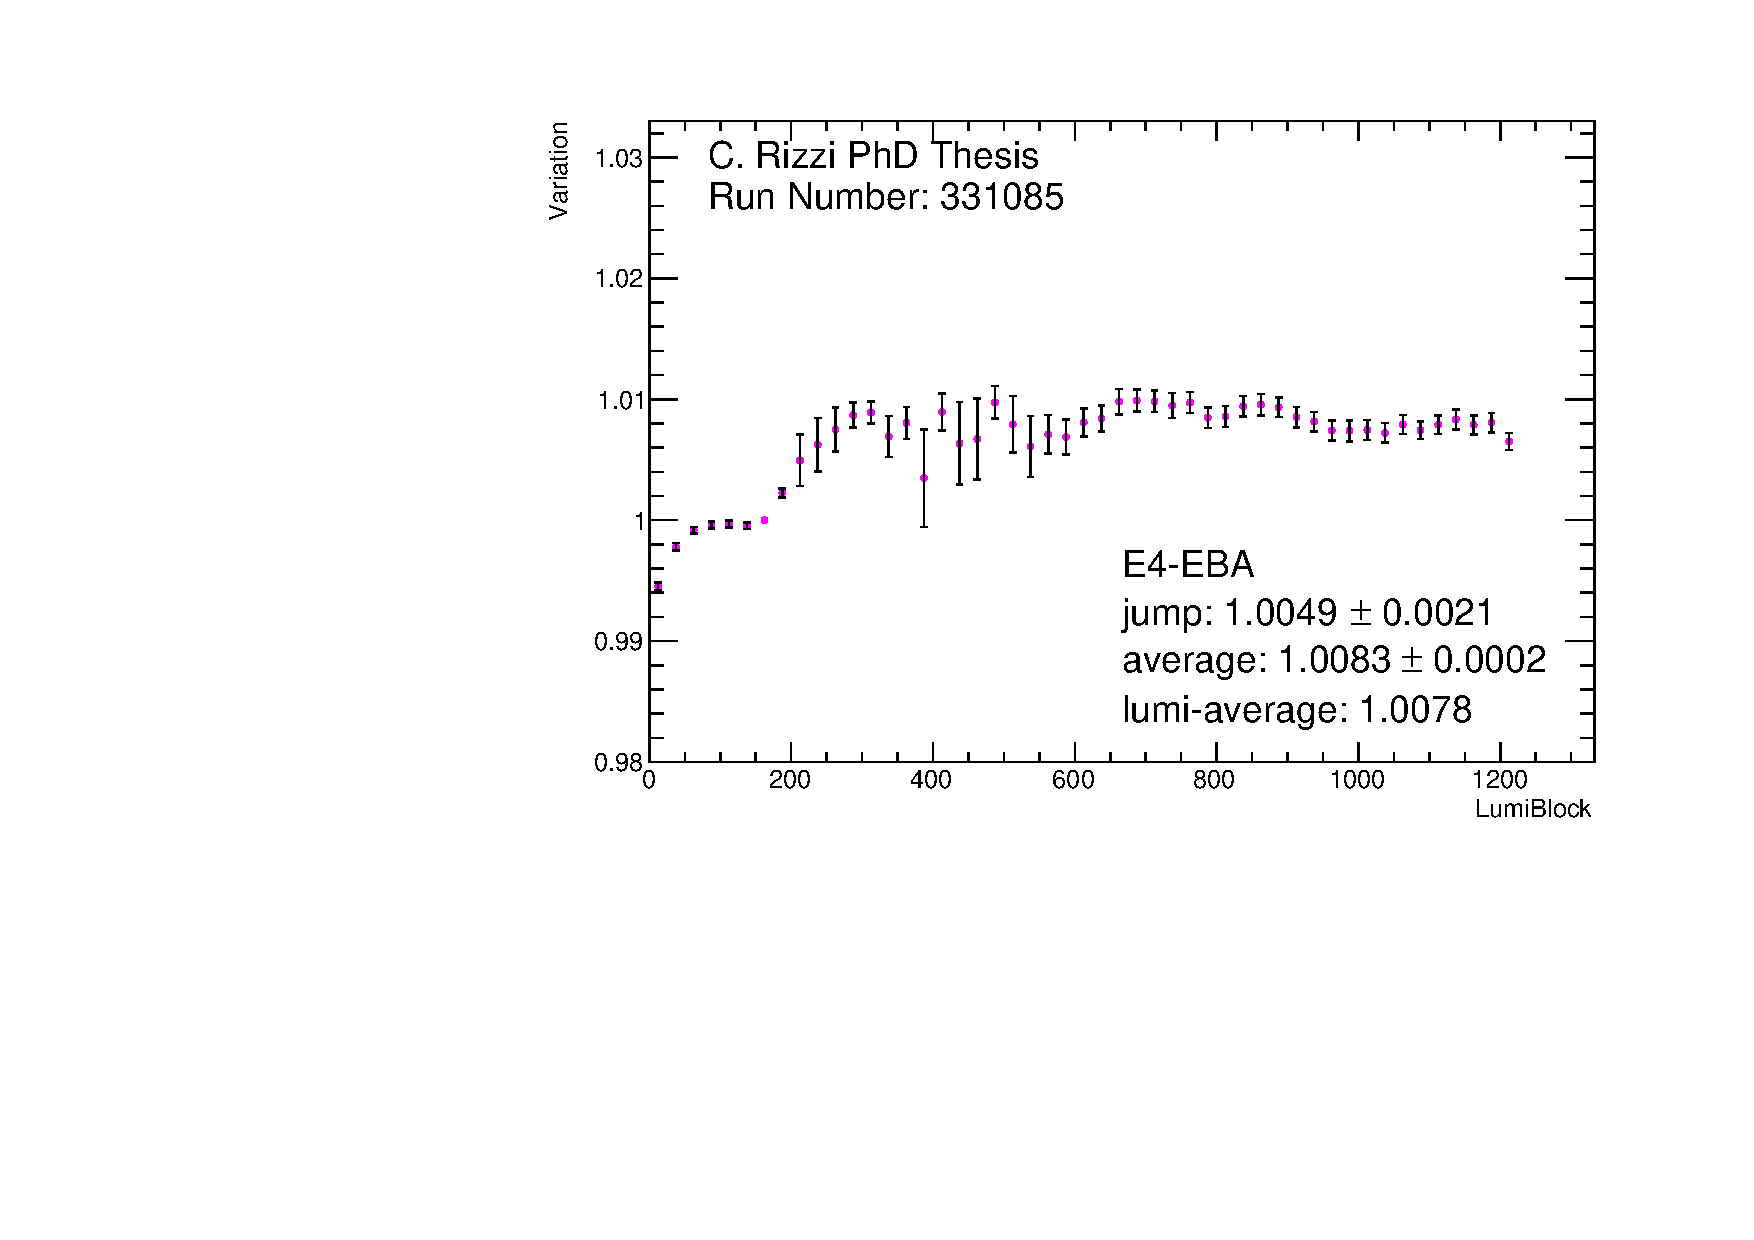
\includegraphics[width=0.45\textwidth]{figures/pmt_response/331085/variation_E4_EBA}\label{fig:app:variation_E4_EBA}}
\subfigure{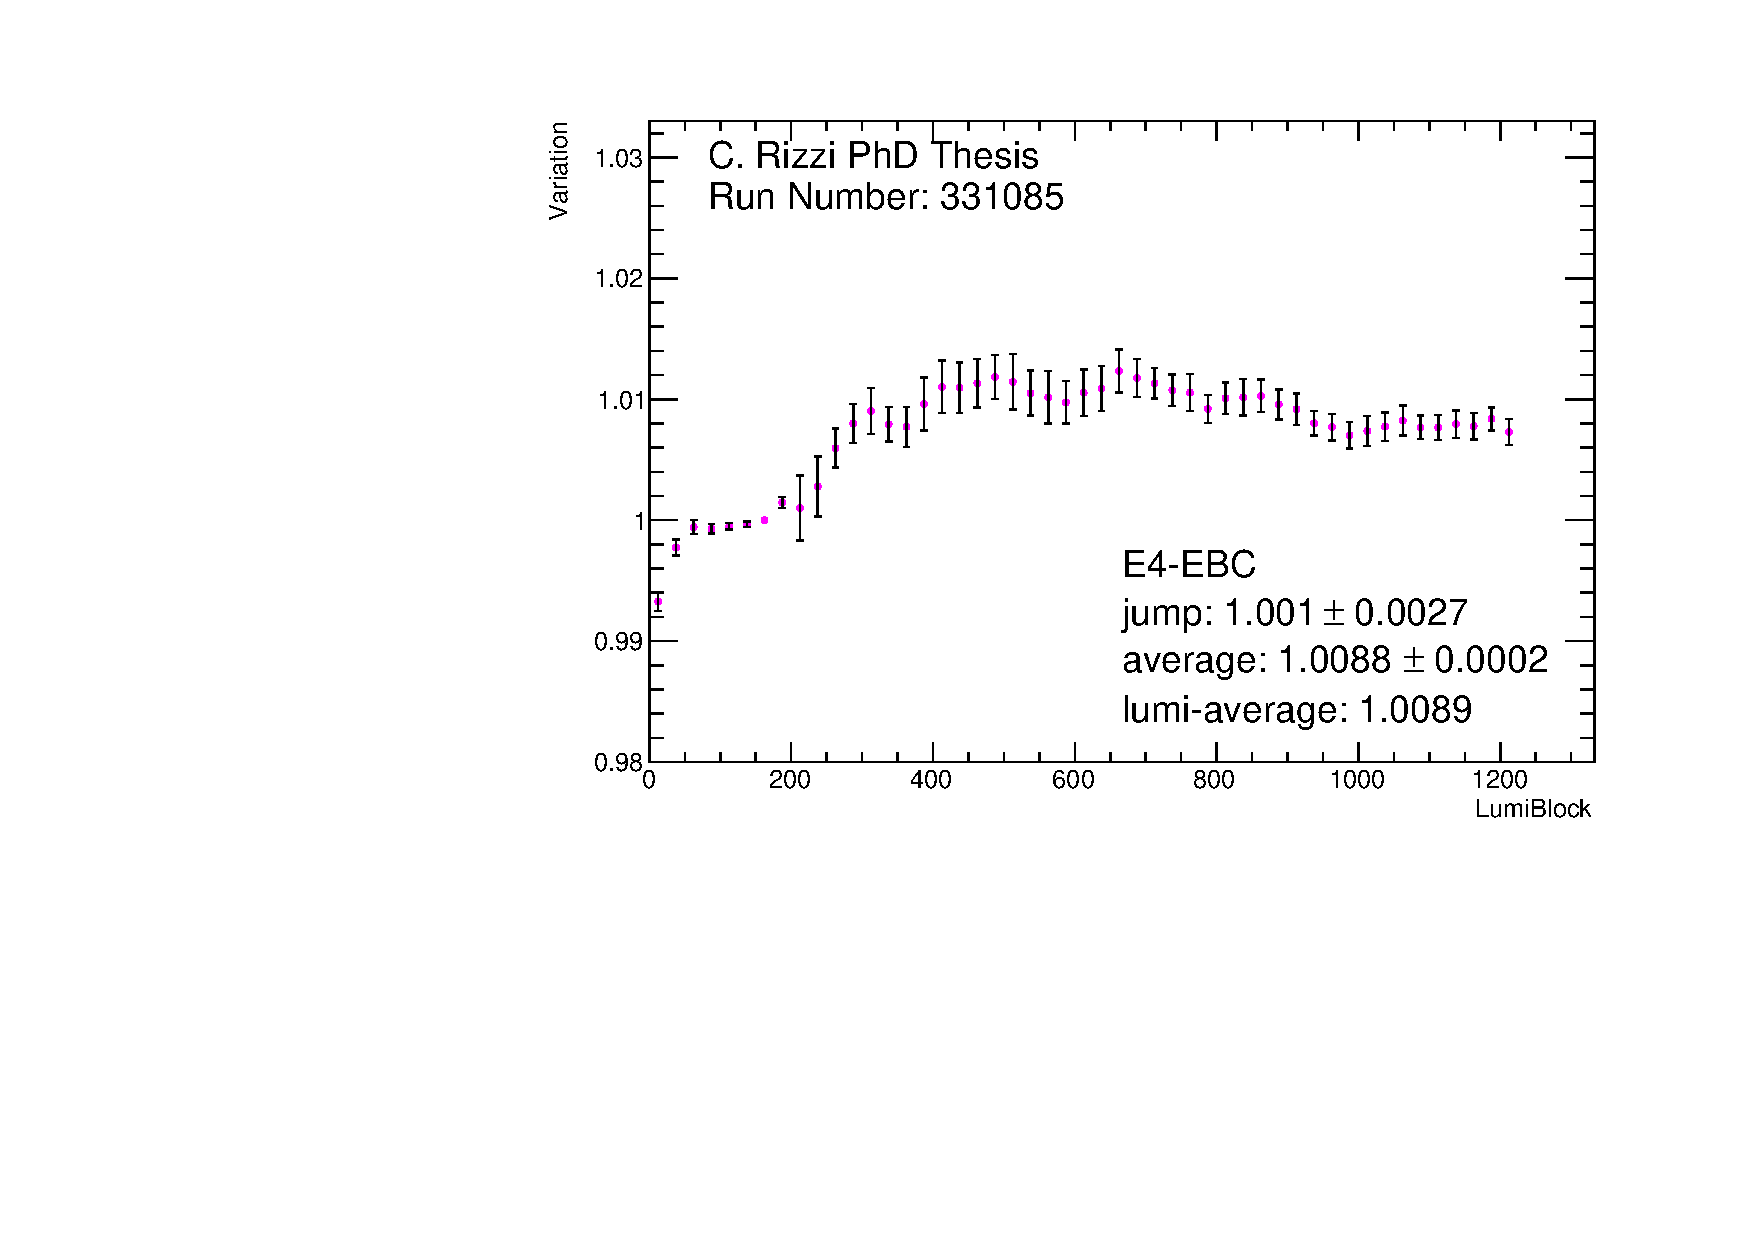
\includegraphics[width=0.45\textwidth]{figures/pmt_response/331085/variation_E4_EBC}\label{fig:app:variation_E4_EBC}}\\
\caption{\gls{pmt} response in cell E3 and E4 for the anchor run (run number 331085).}
\label{fig:apppmt:331085:variation_E3_E4}
\end{figure}

The \gls{pmt} non-linearity is quantified in three different ways, that in the Figures are labeled as:
\begin{description}
\item[Jump] Relative difference between the first group of \glspl{lb} after "stable beams" declaration that does not contain the 
\gls{lb} where "stable beams" is declared and the group of \glspl{lb} used as reference.
\item[Average] Average of the response after "stable beams" is declared until the end of the run, relative to the reference.
\item[Lumi-average] As above, but the average is weighted by the amount of luminosity collected in each group of \glspl{lb}.
\end{description}

\FloatBarrier


\section{Impact on calibration transfer uncertainty}

The change in the \gls{pmt} response with the increase in luminosity has a direct implication in the 
\gls{tilecal} luminosity measurement. 
In particular, it means that the increase in measured current with the increase in luminosity comes from 
two distinct factors:
\begin{itemize}
\item The actual increase in luminosity, i.e. having more particles traversing the detector.
\item The increase in \gls{pmt} response.
\end{itemize}

While the first bullet is the effect that we want to measure to provide a luminosity calibration, 
the second bullet has the effect of artificially increasing the \gls{tilecal} 
luminosity measurement. The value of the \gls{pmt} non-linearity measured in Section \ref{sec:app:pmtresponse} 
is used to correct for this undesired effect, with the net result of \gls{tilecal} providing a higher value 
for the luminosity measurement for the \gls{vdm} run, as schematically illustrated in Figure \ref{fig:apppmt:sketch}.


\begin{figure}[ht]
\centering
\subfigure{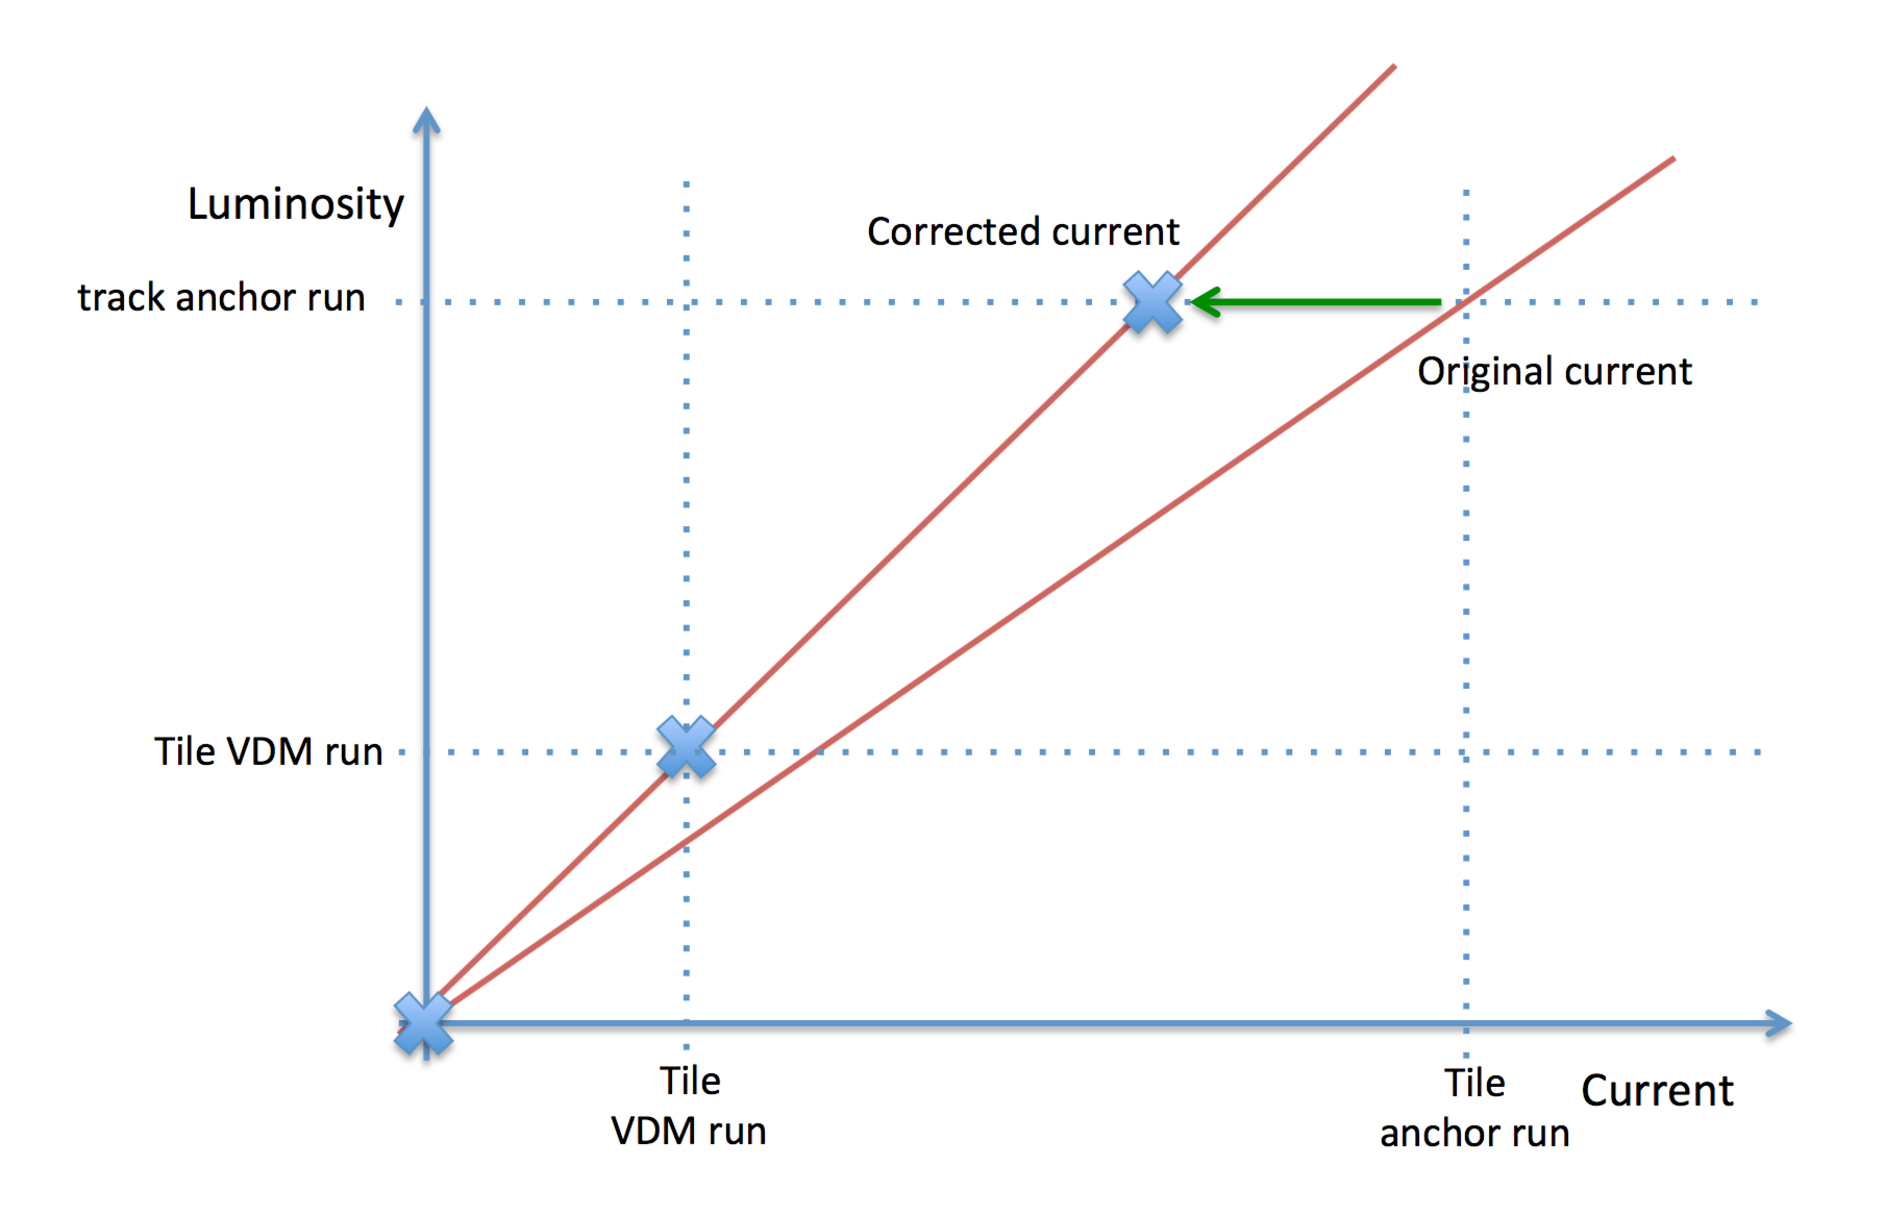
\includegraphics[width=0.65\textwidth]{figures/pmt_response/sketch.pdf}}
\caption{Schematic effect of the correction of the \gls{pmt} response on the \gls{tilecal} luminosity measurement.}
\label{fig:apppmt:sketch}
\end{figure}

\section{Other sources of systematic uncertainty}

\begin{figure}[ht]
\centering
\subfigure{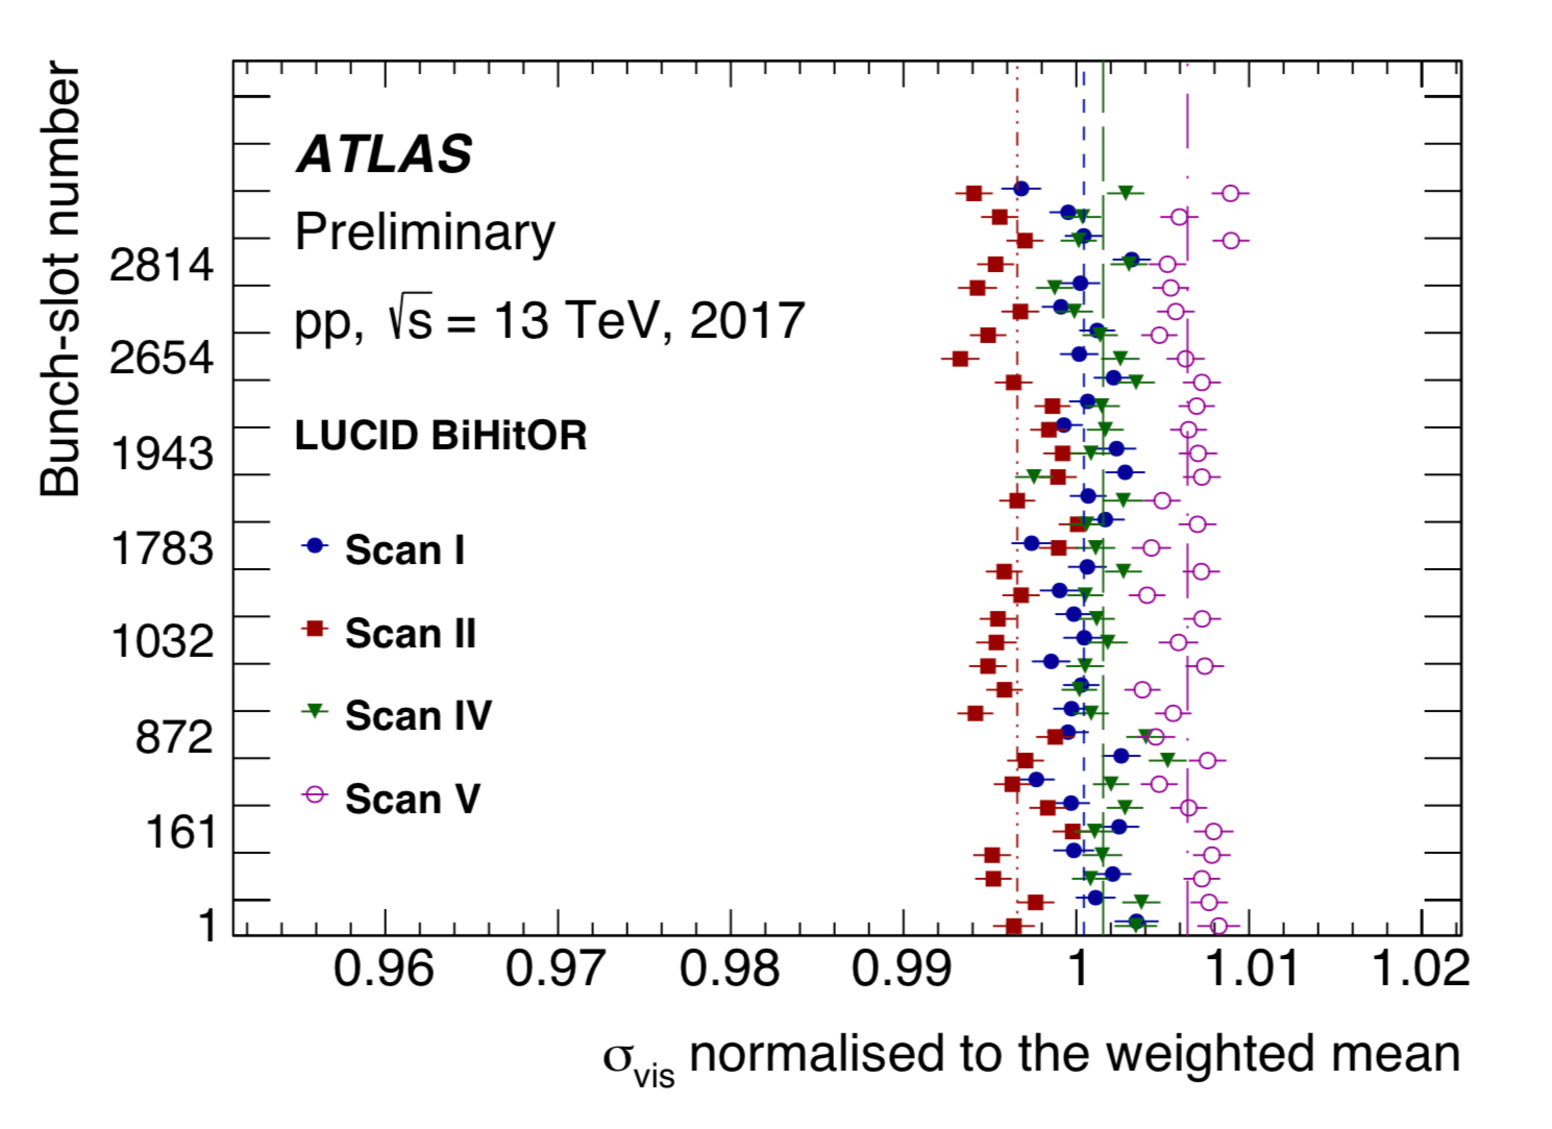
\includegraphics[width=0.43\textwidth]{figures/pmt_response/scan_to_scan.pdf}\label{fig:app:scantoscan}}
\subfigure{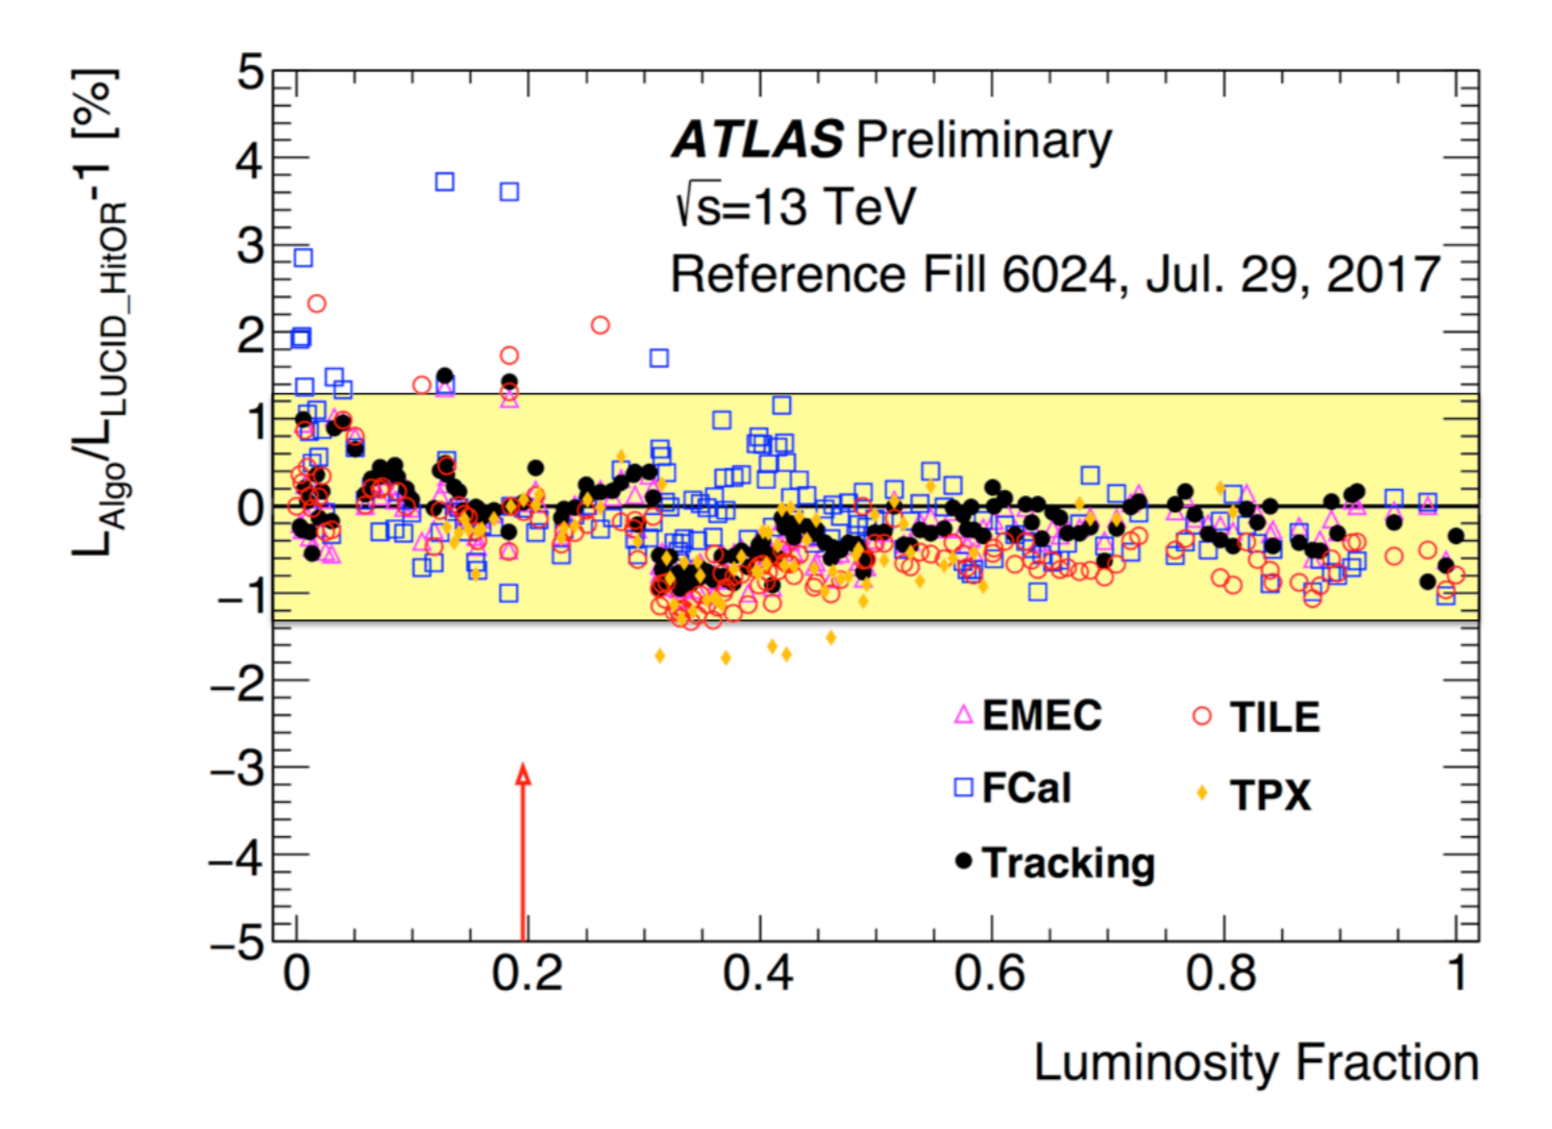
\includegraphics[width=0.55\textwidth]{figures/pmt_response/long_term_stability.pdf}\label{fig:app:longterm}}
\caption{\subref{fig:app:scantoscan} . \subref{fig:app:longterm}}
\label{fig:apppmt:othersyst}
\end{figure}


\section{Conclusion}

The effect a non-linearity in the \gls{pmt} response with the increase in luminosity in the calibration transfer uncertainty from 
\gls{tilecal} has been studies. 
The calibration transfer uncertainty is one of the major sources of uncertainty in the \gls{atlas} luminosity 
measurement, and it has a relevant impact for analyses that rely on a precise luminosity measurement. 
A correction has been derived, that allowed to reduce the calibration transfer uncertainty by XX \%.
This correction has been applied to the computation of the luminosity uncertainty released in March 2018, 
leading to a total luminosity uncertainty of 2.4\% on the 2017 data-taking periods. 


